\documentclass[twoside]{ctuthesis}
\usepackage{array}
\usepackage{textcomp}
\usepackage{xurl}
\usepackage{subcaption}
\usepackage{enumitem}
\usepackage[export]{adjustbox}

\ctusetup{
	titlelanguage = czech,
	mainlanguage = czech,
	otherlanguages = {slovak,english},
	title-czech = {Webová aplikace s~výukovou metodou flash~cards},
	title-english = {Web application with the flash~cards learning method},
	subtitle-czech = {Návrh a~vývoj web aplikace "flash~cards"},
	subtitle-english = {Design and development of "flash~cards" web application},
	doctype = B,
	faculty = F3,
	department-czech = {Katedra počítačů},
	%department-english = {Department of Computer science},
	author = {Lukáš Cafourek},
	supervisor = {Ing. Božena Mannová, Ph.D.},
	%supervisor-address = {Ústav X, \\ Uliční 5, \\ Praha 99},
	%supervisor-specialist = {John Doe},
	%fieldofstudy-english = {Open informatics},
	%subfieldofstudy-english = {Software},
	fieldofstudy-czech = {Otevřená informatika},
	subfieldofstudy-czech = {Software},
	keywords-czech = {flash cards, flashcards, výuka, učení, webová aplikace, aplikace, systematizace výuky, Java, React, SpringBoot, databáze},
	keywords-english = {flash cards, flashcards, education, learning, web application, application, systematization of learning, Java, React, SpringBoot, database},
	day = 21,
	month = 5,
	year = 2025,
	front-specification = true,
	specification-file = {zadani.pdf},
	pkg-hyperref = true,
}

\ctuprocess

\addto\ctucaptionsczech{
	\def\supervisorname{Vedoucí}
	\def\fieldofstudyname{Studijní program}
	\def\subfieldofstudyname{Specializace}
}

\ctutemplateset{maketitle twocolumn default}{
	\begin{twocolumnfrontmatterpage}
		\ctutemplate{twocolumn.thanks}
		\ctutemplate{twocolumn.declaration}
		\ctutemplate{twocolumn.abstract.in.titlelanguage}
		\ctutemplate{twocolumn.abstract.in.secondlanguage}
		\ctutemplate{twocolumn.tableofcontents}
		\ctutemplate{twocolumn.listoffigures}
	\end{twocolumnfrontmatterpage}
}

\begin{abstract-english}
The bachelor's thesis focuses on designing and implementing a web application for the systematization of learning using flash cards.

Functional and non-functional requirements and use cases were defined by analyzing existing solutions. Then, the technologies or tools used were selected, and the application implementation was proposed.

The implementation was followed by its testing, user tests, and deployment. The test results are assessed. In conclusion, the work is evaluated, and further possible development of the web application is mentioned.
\end{abstract-english}

\begin{abstract-czech}
Bakalářská práce je zaměřena na~návrh a~implementaci webové aplikace pro~systematizaci výuky pomocí flash karet.% Implementací a~testováním se bude zabývat pokračující bakalářská práce.

Na~základě provedené analýzy existujících řešení byly definovány funkční a nefunkční požadavky a případy užití. Poté se vybraly použité technologie či nástroje a~navrhla implementace aplikace.

Následovala samotná implementace s~jejím otestováním včetně uživatelských testů a~nasazení aplikace. Výsledky testování jsou posouzeny. V~závěru je práce zhodnocena a~je zmíněn možný další vývoj webové aplikace.
\end{abstract-czech}

% Acknowledgements / Podekovani
\begin{thanks}
Chtěl bych poděkovat Ing.~Boženě~Mannové,~Ph.D. za~vedení mé bakalářské práce včetně poskytnutých konzultací a~užitečných rad. Dále bych chtěl poděkovat rodině, přátelům i~kolegům studentům za~jejich podporu.
\end{thanks}

% Declaration / Prohlaseni
\begin{declaration}
Prohlašuji, že jsem bakalářskou práci vypracoval samostatně a~že jsem uvedl veškerou použitou literaturu, v~souladu s~Metodickým pokynem o~dodržování etických principů při~přípravě vysokoškolských závěrečných prací a~Rámcovými pravidly používání umělé inteligence na~ČVUT pro~studijní a~pedagogické účely v~Bc a~NM studiu..

\medskip

V~Praze, \ctufield{day}.~\monthinlanguage{title}~\ctufield{year}
\end{declaration}

\begin{document}

\maketitle

\floatstyle{plaintop}
\restylefloat{table}

\chapter{Úvod}

\section{Téma}

Tématem bakalářské práce je návrh a~implementace webové aplikace pro~systematizaci výuky pomocí karet, které obsahují na~jedné straně definici či otázku a~na~druhé její vysvětlení nebo odpověď. Aplikace flash cards je určena k~podpoře přípravy na~zkoušky, testy, výuku cizích jazyků či další různé látky studia. Uživatelům nabídne možnost efektivně a~snadno spravovat vlastní sety karet v~uživatelsky přívětivém rozhraní, čímž se usnadní proces studia a~zlepší se organizační struktura vzdělávacích materiálů.

\section{Motivace}

Flash karty představují účinný nástroj pro~zapamatování a systematické osvojování jednotlivých částí studijních materiálů~\cite{maine}, což mohu potvrdit z~vlastní zkušenosti. Digitalizace výukového systému pomocí metody flash karet pomůže k~efektivnější přípravě na~vysokoškolské zkoušky a testy. Cílem práce je provést rešerši existujících řešení, navrhnout implementaci webové aplikace pro~tento účel a~realizovat ji. Sloužit má především studentům, jimž aplikace usnadní průběh studia.

\chapter{Rešerše}

V~této kapitole je popsáno, co jsou flash karty a~jak jsou využívány při~studiu, a~rozebráno pět vybraných dostupných webových aplikací využívajících tuto metodu výuky.

\section{Flash cards}

Učební metoda memorizace s~použitím flash karet spočívá v~otázce na~jedné straně a~odpovědi na~druhé straně karty. Nejčastěji se metoda využívá jako oblíbený nástroj ke~studiu cizích slov, ale dokáže zlepšit výuku i~v~jiných odvětvích.

Běžně se vytváří fyzické karty pro~žáky a~studenty, na~něž je potřeba prakticky jen papír a~tužka, což značí velkou výhodu v~jednoduchém, všestranném a~levném učení. Člověk se může učit odkudkoliv, jelikož jsou karty skladné, a~lze si vytvářet kolekce kartiček pro~různé předměty ve~studiu~\cite{twinkl, poustka}.

Flash karty umožňují opakovat si potřebné informace v~různých částech dne. Místo prohlížení studijních materiálů si člověk paměť procvičuje aktivní memorizací i~několikrát denně. Tím se danou informaci může naučit dříve a~efektivněji než z~pasivních materiálů, ať už z~prezentací, skript nebo dokumentů. Jelikož jsou studijní materiály rozdělené do~několika karet, jednotlivec se vyhýbá souvislému textu a~dlouhému čtení. Také se díky kartám může více zaměřit na~studijní látku, kterou si ještě tolik nepamatuje, a~dané otázky více opakovat~\cite{maine}.

Důležité je vytvořit si kolekci karet pro každou kategorii studované látky, aby se karty skládaly jen z~dílčích informací. Každý by si měl vytvořit karty přímo pro~sebe, například s~použitím obrázků či různých hesel. Nejdříve je dobré odpovědět nahlas na~otázku bez~odhalení popisu definice na~druhé straně karty. Ovšem při~neúspěchu odpovědi si člověk využívající papírové kartičky může danou kartu z~kolekce dát do~spodu balíčku pro~další iteraci učení nebo si ji dát do~separátního balíčku dané kolekce otázek nutných k~častější memorizaci. Hlavním bodem metody je často opakovat a~studovat~\cite{maine}.

\newpage

Podle teorie „křivky zapomínání“ Hermanna Ebbinghause si člověk při~prvním učení informace uchovává po~krátkou dobu. S~postupem času však zapomíná rychleji. Rozložené opakování (angl. spaced repetition) je jednou ze~strategií, jíž může každý využít, aby zabránil ztrátě naučených informací a~začal si je ukládat do~dlouhodobé paměti. Rozložené opakování funguje následujícím způsobem~\cite{twinkl}:

\begin{itemize}
\item Studovat informaci
\item Přejít na~něco jiného
\item Znovu se k~informacím později vrátit
\item Proces opakovat
\end{itemize}

Nevýhodou fyzických papírových karet je především větší práce s~jejich vytvářením a nebezpečí jejich ztráty. Upravovat již vytvořené karty je složité a~často člověk místo toho vytvoří kartu novou. Mimo~textových odpovědí je těžké přidávat k~nim obrázky, schémata nebo audiovizuální informace. Digitální aplikace pomáhají tyto nevýhody odstranit.

\renewcommand{\arraystretch}{1.5}

\section{Zvolená existující řešení}

Zde jsou analyzovány funkcionality a~případy užití některých existujících aplikací včetně jejich výhod a~nevýhod. Na~trhu existuje mnoho aplikací, níže je popsáno pět nejpoužívanějších, nejpopulárnějších a~nejdostupnějších. Důležité poznatky jsou na~konci shrnuty a~porovnány. Vedle~aplikací webových se objevují i~desktopové pro~počítače a~mobilní pro~Android a~iOS.

\subsection{Quizlet}

Quizlet je jednou z~nejpopulárnějších aplikací s~metodou výuky flash karet. Vyznačuje se velmi přívětivým uživatelským rozhraním a~nejvíce mimikuje tradiční papírové flash karty.

Po~registraci uživatel může tvořit své vlastní sety karet, které si libovolně upravuje dle~svých představ. Mimo textových vstupů může člověk využít také obrázky. Pokud je nutné učit se například cizí slova, Quizlet nabízí poslechnout si strojové nahrávky, na něž je možnost napsat odpověď. Uživatel si může vybrat z~předpřipravených sad flash karet. Toto vše je v~aplikaci zpoplatněno včetně sdílení setů karet a~využití Quizlet umělé inteligence k~podpoře výuky. Bez~předplatného se uživateli zobrazuje reklama a~může pouze tvořit sety karet s~textovými vstupy~\cite{tsay, ransom}.

\newpage

Formu učení si lze vybrat z~více možností, mezi~něž patří klasické flash karty nebo vyplňování testů, které Quizlet sám připraví. Při~zapnutí systémových oznámení aplikace upozorňuje, že je čas opět studovat daný set flash karet. Uživatel si vytvoří učební plán, jak dlouho a~jaké sety se chce denně učit. U~každé flash karty je možno pojem zařadit mezi těžší, a~tím se bude otázka častěji opakovat v~probíraném setu~\cite{quizlet}. Uvedená tabulka~\ref{tab:quiz} shrnuje výhody a~nevýhody aplikace Quizlet.

\begin{table}[H]
\caption{Výhody a nevýhody aplikace Quizlet}
\begin{tabular}{| >{\centering\arraybackslash}m{5cm} | >{\centering\arraybackslash}m{5cm} |}
\hline
\textbf{Výhody} & \textbf{Nevýhody} \\ \hline
Prakticky na~všech nejpoužívanějších platformách & Mnoho funkcí s~předplatným \\ \hline
Jednoduché uživatelské rozhraní  & \\ \hline
Velký počet výukových forem  & \\ \hline
Možnost využívat umělou inteligenci  & \\ \hline
\end{tabular}
\label{tab:quiz}
\end{table}

\subsection{Cram}

Cram je jednoduchá flashcard aplikace se~zajímavými efektivními funkcemi. Uživatel si může vytvořit sety karet i~s~použitím obrázků~\cite{ransom}.

Uživatel může přidat ke~kartě nápovědu, což může dobře simulovat reálného zkoušejícího člověka. Aplikace má standardní formu učení pomocí otáčení karet. Otázky, na~něž člověk správně odpoví, se v~budoucnu neobjevují v~setu. To může být prospěšné pro~časté učení, kdy se student nemusí zatěžovat otázkami, na~které zná odpovědi\cite{ransom, cram}.

Kromě klasického otáčení flash karet aplikace umožňuje vyplňování testů včetně true/false odpovědí a~výběru z více možností. Uživatel si může zahrát dvě studijní hry, které mohou být prospěšné hlavně pro malé žáky a~žačky. Bez placené verze se zobrazuje reklama a~jsou znepřístupněny pokročilé formátovací funkce flash karet~\cite{ransom, cram}. Uvedená tabulka~\ref{tab:cr} shrnuje výhody a~nevýhody aplikace Cram.

\newpage

\begin{table}[H]
\caption{Výhody a nevýhody aplikace Cram}
\begin{tabular}{| >{\centering\arraybackslash}m{5cm} | >{\centering\arraybackslash}m{5cm} |}
\hline
\textbf{Výhody} & \textbf{Nevýhody} \\ \hline
Prakticky na~všech nejpoužívanějších platformách & Méně pokročilých funkcí \\ \hline
Jednoduché uživatelské rozhraní  & Zastaralé uživatelské rozhraní \\ \hline
Velký počet předpřipravených setů karet  & \\ \hline
Možnost studijních her & \\ \hline
\end{tabular}
\label{tab:cr}
\end{table}

\subsection{Anki}

Anki je všestranná aplikace, jež velmi dobře využívá svůj algoritmus rozloženého opakování (AnkiApp Advanced Spaced Repetition\texttrademark{}) pro~efektivní studium. Mnoho webů doporučuje aplikaci jako nejlepší volbu pro~studium metodou flash karet, což umocňuje kvalitu výukové metody a~synchronizace mezi všemi zařízeními, ačkoli Anki disponuje méně přívětivým uživatelským rozhraním~\cite{ransom, anki}.

Aplikace je kompletně zdarma (kromě iOS aplikace) a~open-source. Standardně si uživatel vytváří sady flash karet a~učení spočívá v~jejich otáčení. Po~zodpovězení otázky si uživatel určí, jak byla otázka obtížná. Podle zvolené obtížnosti ji Anki chytře zařadí do setu karet, aby se uživateli znovu ukázala dříve či později. To může znamenat několik minut nebo pár měsíců. Toto je velmi účinné, protože člověk znovu narazí na otázku, kterou už skoro zapomněl, a~tím si ji zopakuje. Také se uživatel nezatěžuje jednoduchými otázkami~\cite{poustka, ransom}.

Uživatel může využít i~předpřipravené sety karet a~přidávat obrázky i~audio vstupy k~samotným kartám. Celé studium se dá zobrazit pomocí statistik, jež mohou i~motivovat do~dalšího učení~\cite{anki}. Uvedená tabulka~\ref{tab:an} shrnuje výhody a~nevýhody aplikace Anki.

\begin{table}[H]
\caption{Výhody a nevýhody aplikace Anki}
\begin{tabular}{| >{\centering\arraybackslash}m{5cm} | >{\centering\arraybackslash}m{5cm} |}
\hline
\textbf{Výhody} & \textbf{Nevýhody} \\ \hline
Prakticky na~všech nejpoužívanějších platformách & Neintuitivní uživatelské rozhraní \\ \hline
Zcela zdarma (kromě iOS) & \\ \hline
Velký počet předpřipravených setů karet  & \\ \hline
Velmi efektivní algoritmus metody flash cards & \\ \hline
\end{tabular}
\label{tab:an}
\end{table}

\subsection{Brainscape}

Brainscape vypadá jako jednoduchá aplikace, která ovšem nabízí pokročilé funkce rozloženého opakování (Confidence-Based Repetition) pro~účinné studium pomocí metody flash karet~\cite{ransom, brainscape}.

Startem je vytvoření třídy, do~níž se vytváří sety karet. Samotné karty se snadno v~aplikaci vytváří ovšem s~tím rozdílem, že otázka i odpověď jsou na~stejné straně, jen v~jiném sloupci. Odpověď je ale skryta, dokud ji člověk sám neodkryje. Pokud chce uživatel přidávat cokoli jiného než~text, musí si předplatit Pro verzi aplikace~\cite{ransom}.

Po~odkrytí odpovědi na~otázku se Brainscape zeptá na~obtížnost otázky, podobně jako Anki. Podle toho danou otázku zařadí do~dalších iterací učení vícekrát či méněkrát než~doposud. Podle zhodnocení otázek Brainscape přiřazuje danému setu karet procentuální dokončení setu a~uživatele informuje o~dalším studiu setu, dokud není celý set označen sty procenty~\cite{ransom}. Uvedená tabulka~\ref{tab:brain} shrnuje výhody a~nevýhody aplikace Brainscape.

\begin{table}[H]
\caption{Výhody a nevýhody aplikace Brainscape}
\begin{tabular}{| >{\centering\arraybackslash}m{5cm} | >{\centering\arraybackslash}m{5cm} |}
\hline
\textbf{Výhody} & \textbf{Nevýhody} \\ \hline
Prakticky na~všech nejpoužívanějších platformách & Mnoho funkcí za~předplatným \\ \hline
Jednoduché uživatelské rozhraní & \\ \hline
Efektivní algoritmus metody flash cards & \\ \hline
\end{tabular}
\label{tab:brain}
\end{table}

\subsection{Kahoot!}

Kahoot! je známá aplikace, kterou učitelé rádi využívají jako podporu své výuky. Je přizpůsobena pro~mladší uživatele a~učení velmi zpříjemňuje herním stylem a~módy. Uživatelé také mezi sebou mohou soutěžit získáváním bodů na~základě rychlosti a~správnosti odpovědí.

Kahoot! nabízí množství různých studijních módů, mezi~něž patří hlavně kvízy s~výběrem z~více možností a~true/false odpověďmi. Metodu flash karet přidali před~pěti lety, a~tím rozšířili pole působnosti na~trhu. Uživatel může sety karet tvořit a~vybírat z~již vytvořených setů jiných lidí, pokud jsou zdarma. Když si uživatel předplatí některý z~plánů, odemkne si další funkcionality, jež mu pomohou při~studiu. Mezi~ně patří AI generátor z~PDF dokumentu nebo jiných zdrojů, přidávání obrázků nebo audiovizuálních vstupů ke~kartám, statistiky učení, čtyři herní módy a~sdílení setů s dalšími lidmi používajících aplikaci~\cite{kahoot, kahoot-plan}.

\newpage

Mnoho funkcí je dostupných s~předplatnými, které jsou celkem čtyři. V~bezplatné verzi se nemůže člověk vracet k~odpovězeným otázkám, nefunguje žádný algoritmus pro~více či méně opakování otázek, jež uživatel studoval, a~nefungují funkce zmíněné v~poslední větě minulého odstavce. Předplatná jsou velmi drahá, ale zahrnují v~sobě i~další funkce pro~jiné studijní metody, než jsou flash karty~\cite{kahoot, kahoot-plan}. Uvedená tabulka \ref{tab:kah} shrnuje výhody a~nevýhody aplikace Kahoot!

\begin{table}[H]
\caption{Výhody a nevýhody aplikace Kahoot!}
\begin{tabular}{| >{\centering\arraybackslash}m{5cm} | >{\centering\arraybackslash}m{5cm} |}
\hline
\textbf{Výhody} & \textbf{Nevýhody} \\ \hline
Prakticky na~všech nejpoužívanějších platformách & Mnoho funkcí je předplaceno \\ \hline
Jednoduché uživatelské rozhraní & Drahá cena předplatných \\ \hline
Mnoho herních módů & \\ \hline
Velký počet výukových forem  & \\ \hline
Možnost využívat umělou inteligenci  & \\ \hline
\end{tabular}
\label{tab:kah}
\end{table}

\newpage

\subsection{Shrnutí}

Byla provedena analýza pěti aplikací na trhu Quizlet, Cram, Anki, Brainscape a~Kahoot! Z~poznatků je sestavena následující tabulka~\ref{tab:shrnuti}, v~níž se shrnula a~porovnala jednotlivá řešení.

\begin{table}[H]
\caption{Souhrnné srovnání flashcard aplikací}
\centering
\begin{tabular}{| >{\centering\arraybackslash}m{2cm} | >{\centering\arraybackslash}m{2.17cm} | >{\centering\arraybackslash}m{1.74cm} | >{\centering\arraybackslash}m{1.87cm} | >{\centering\arraybackslash}m{2.17cm} | >{\centering\arraybackslash}m{2.17cm} |}
\hline
 & \textbf{Quizlet} & \textbf{Cram} & \textbf{Anki} & \textbf{Brainscape} & \textbf{Kahoot!} \\ \hline
\textbf{Platforma} & Web, Android, iOS & Web, Android, iOS & Web, PC, Android, iOS & Web, Android, iOS & Web, Android, iOS \\ \hline
\textbf{Předplatné} & Ano (686~Kč/rok) & Ano (\$9.95/rok) & Ne (pouze iOS \$24.99) & Ano (\$7.99/rok nebo \$199.99) & Ano (\$58.49--\$290.49/rok) \\ \hline
\textbf{Verze zdarma} & Ano, málo funkcí & Ano, reklamy & Ano & Ano, málo funkcí & Ano, málo funkcí \\ \hline
\textbf{Reklamy} & Ano, verze zdarma & Ano, verze zdarma & Ne & Ne & Ne \\ \hline
\textbf{Interface} & Jednoduchý & Zastaralý & Neintuitivní & Jednoduchý & Jednoduchý \\ \hline
\textbf{Rozložené opakování} & Ano & Ne & Ano & Ano & Ano, s~předplatným \\ \hline
\textbf{Režimy výuky} & Ano & Ano & Ano & Ano & Ano \\ \hline
\textbf{Šablony} & Ano & Ano & Ano & Ano & Ano \\ \hline
\textbf{Před\-připravené sety} & Ano, většina s~předplatným & Ano & Ne & Ano & Ano, většina s~předplatným \\ \hline
\textbf{Pokročilé funkce} & Ano, s~předplatným & Ano, málo & Ano & Ano, s~předplatným & Ano, s~předplatným \\ \hline
\textbf{Statistiky} & Ano & Ano & Ano & Ano & Ano, s~předplatným \\ \hline
\textbf{Multi\-média} & Ano, s~předplatným & Ano & Ano & Ano, s~předplatným & Ano, s~předplatným \\ \hline
\textbf{Cloud sync} & Ano & Ano & Ano & Ano & Ano \\ \hline
\textbf{Umělá inteligence} & Ano, s~předplatným & Ne & Ne & Ne & Ano, s~předplatným \\ \hline
\end{tabular}
\label{tab:shrnuti}
\end{table}

\chapter{Analýza}

V~této kapitole je provedena analýza, která pomůže pochopit fungování aplikace a~poté výběr technologie či nástroje k~návrhu a~realizaci její implementace. Obrázky diagramů byly vytvořeny v~nástroji Enterprise Architect~15~\cite{ea}.

\section{Specifikace požadavků}

Na~základě předešlé rešerše, zadání práce a~autorova vlastního přesvědčení je v~této sekci rozebrána analýza a~sběr požadavků pro~návrh vlastní webové aplikace flash karet.

Potřebné požadavky jsou roztříděny na~funkční a~nefunkční.

\subsection{Funkční požadavky}

Funkční požadavky definují specifikace, jež popisují funkcionality aplikace. Jedná se o~konkrétní požadavky, které navrhnutá webová aplikace musí splňovat a~poskytovat, aby se naplnily cíle práce~\cite{frnfr}. Funkční požadavky jsou označeny jako \emph{FRn -- název}, kde \emph{n} znamená číslo požadavku. Požadavky jsou znázorněny v~obrázku~\ref{fig:fr} níže.

\begin{figure}[H]
\centering
\includegraphics[width=1\textwidth]{Funkční Požadavky.png}
\caption{Funkční požadavky}
\label{fig:fr}
\end{figure}

\newpage

\begin{itemize}
\item \textbf{FR01 -- Registrace a přihlášení} 

Aplikace umožní uživateli registrovat se a~přihlašovat pomocí e-mailu a~hesla, jež se musí skládat alespoň z~jednoho velkého a~malého písmena, číslice a~speciálního znaku.

\item \textbf{FR02 -- Obnova zapomenutého hesla}

Aplikace umožní uživateli obnovit si zapomenuté heslo tím, že na~zaregistrovaný e-mail bude zaslána zpráva s~kódem s~časovou platností, který vloží do aplikace a~vytvoří si heslo nové.

\item \textbf{FR03 -- Správa setů flash karet}

Aplikace umožní uživateli vytvářet si, upravovat a~mazat osobní sady flash karet.

\item \textbf{FR04 -- Správa flash karet}

Aplikace umožní uživateli vytvářet si, upravovat a~mazat flash karty v~rámci osobní sady.

\item \textbf{FR05 -- Přidávání obrázků}

Aplikace umožní uživateli kromě textových vstupů přidávat i~obrázky jako obsah flash karet.

\item \textbf{FR06 -- Filtrace a vyhledávání setů karet}

Aplikace umožní uživateli filtrovat a~vyhledávat v~osobních i~veřejných setech podle jména setu nebo kategorie, v~níž se set nachází.

\item \textbf{FR07 -- Statistika učení}

Aplikace umožní uživateli vidět svou statistiku výuky, tzn. kolik setů celkově prošel a~kolikrát jednotlivé sety flash karet studoval a další.

\item \textbf{FR08 -- Sdílení setů}

Aplikace umožní uživateli označit si set jako veřejný, jenž bude dostupný i~pro~ostatní uživatele. Spravovat daný set bude moci pouze autor. 

\item \textbf{FR09 -- Oblíbené sety flash karet}

Aplikace umožní uživateli označit si své i~veřejné sety jako oblíbené, aby je mohl snadněji najít v~seznamu oblíbených setů.

\item \textbf{FR10 -- Formátování textu flash karet}

Aplikace umožní uživateli u~každé flash karty psaný text formátovat pro~detailnější a~čitelnější popis.

\item \textbf{FR11 -- Režimy výuky}

Aplikace umožní uživateli studovat set flash karet standardní metodou, vybíráním z~více možností nebo označením pravda/nepravda.

\item \textbf{FR12 -- OAuth2 přihlášení}

Aplikace umožní uživateli registrovat se a~přihlašovat pomocí Google účtu.
\end{itemize}

\subsection{Nefunkční požadavky}

Nefunkční požadavky definují specifikace, jež se spojují s~výkonem, architekturou, bezpečností a~dalšími. Nespojují se přímo s~požadavky funkcionalit aplikace~\cite{frnfr}. Nefunkční požadavky jsou označeny jako \emph{NFRn -- název}, kde \emph{n} znamená číslo požadavku. Požadavky jsou znázorněny na~obrázku~\ref{fig:nfr} níže.

\begin{figure}[H]
\centering
\includegraphics[width=1\textwidth]{Nefunkční Požadavky.png}
\caption{Nefunkční požadavky}
\label{fig:nfr}
\end{figure}

\begin{itemize}
\item \textbf{NFR01 -- Responzivní uživatelské rozhraní}

Rozhraní se vytvoří jako Single Page Application s~využitím technologie React pro~plynulé a~responzivní prostředí. Aplikace musí být dostupná na~PC i~mobilních zařízeních.

\item \textbf{NFR02 -- Použití Spring Boot}

Pro~komunikaci se serverem se využije Java Spring Boot, což umožní snažší správu a~konfiguraci projektu.

\item \textbf{NFR03 -- Hibernate jako ORM}

Java knihovna Hibernate se použije pro~objektově relační mapování (angl. Object-Relational Mapping), což usnadňuje zachování a~přístup k~datům z~databáze aplikace.

\item \textbf{NFR04 -- Ukládání do SQL databáze}

Aplikace musí persistentně ukládat všechna potřebná data do~SQL relační databáze.

\item \textbf{NFR05 -- Kompatibilita}

Klientská část aplikace musí být kompatibilní se~všemi nejpoužívanějšími webovými prohlížeči Chrome, Edge, Safari a~Firefox.

\newpage

\item \textbf{NFR06 -- Rychlost aplikace}

Serverová část aplikace musí být dostatečně rychlá, aby uživatel v~aplikaci zbytečně nečekal na~načtení všech objektů z~databáze.

\item \textbf{NFR07 -- Bezpečnost aplikace}

Aplikace musí využívat zabezpečenou komunikaci prostřednictvím šifrování protokolem HTTPS. Data musí být chráněna, uživatelé při~přihlašování ověřováni a~hesla hashována.

\item \textbf{NFR08 -- Jazyk a srozumitelnost aplikace}

Rozhraní aplikace bude v~angličtině a~musí být srozumitelné pro~uživatele všech kategorií, aby bylo snadné aplikaci používat.

\item \textbf{NFR09 -- Vývoj a údržba}

Aplikace musí být zdokumentována pro~další vývoj a~údržbu. Jedná se také o~použití různých design patternů a~srozumitelnost kódu.
\end{itemize}

\section{Případy užití}

Tato sekce je zaměřena na~případy užití a~jejich aktéry. Případy slouží k~detailnímu popisu různých interakcí aktérů se~systémem a~používání jednotlivých funkcí. Mezi aktéry lze zařadit nejen reálné uživatele, ale i~různé části nebo procesy systému (například automatické posílání e-mailů).% V~první podsekci zmiňujeme samotné aktéry aplikace a~v~další uvádíme obrázek případů užití.

\subsection{Aktéři}

Analýzou a~specifikací požadavků v~minulé podkapitole byli identifikováni tři různí aktéři aplikace:
\begin{enumerate}
\item \textbf{Nepřihlášený uživatel}

Reprezentuje uživatele, který je nepřihlášen nebo nezaregistrován.

\item \textbf{Přihlášený uživatel}

Reprezentuje uživatele, který má vytvořen účet v~aplikaci a~je přihlášen.

\item \textbf{Systém}

Reprezentuje posílání notifikací a~zpráv na~e-mail uživatele.
\end{enumerate}

\newpage

\subsection{Diagram případů užití}

Níže se nachází detailní obrázek~\ref{fig:uc} případů užití aplikace včetně všech aktérů.

\begin{figure}[H]
\centering
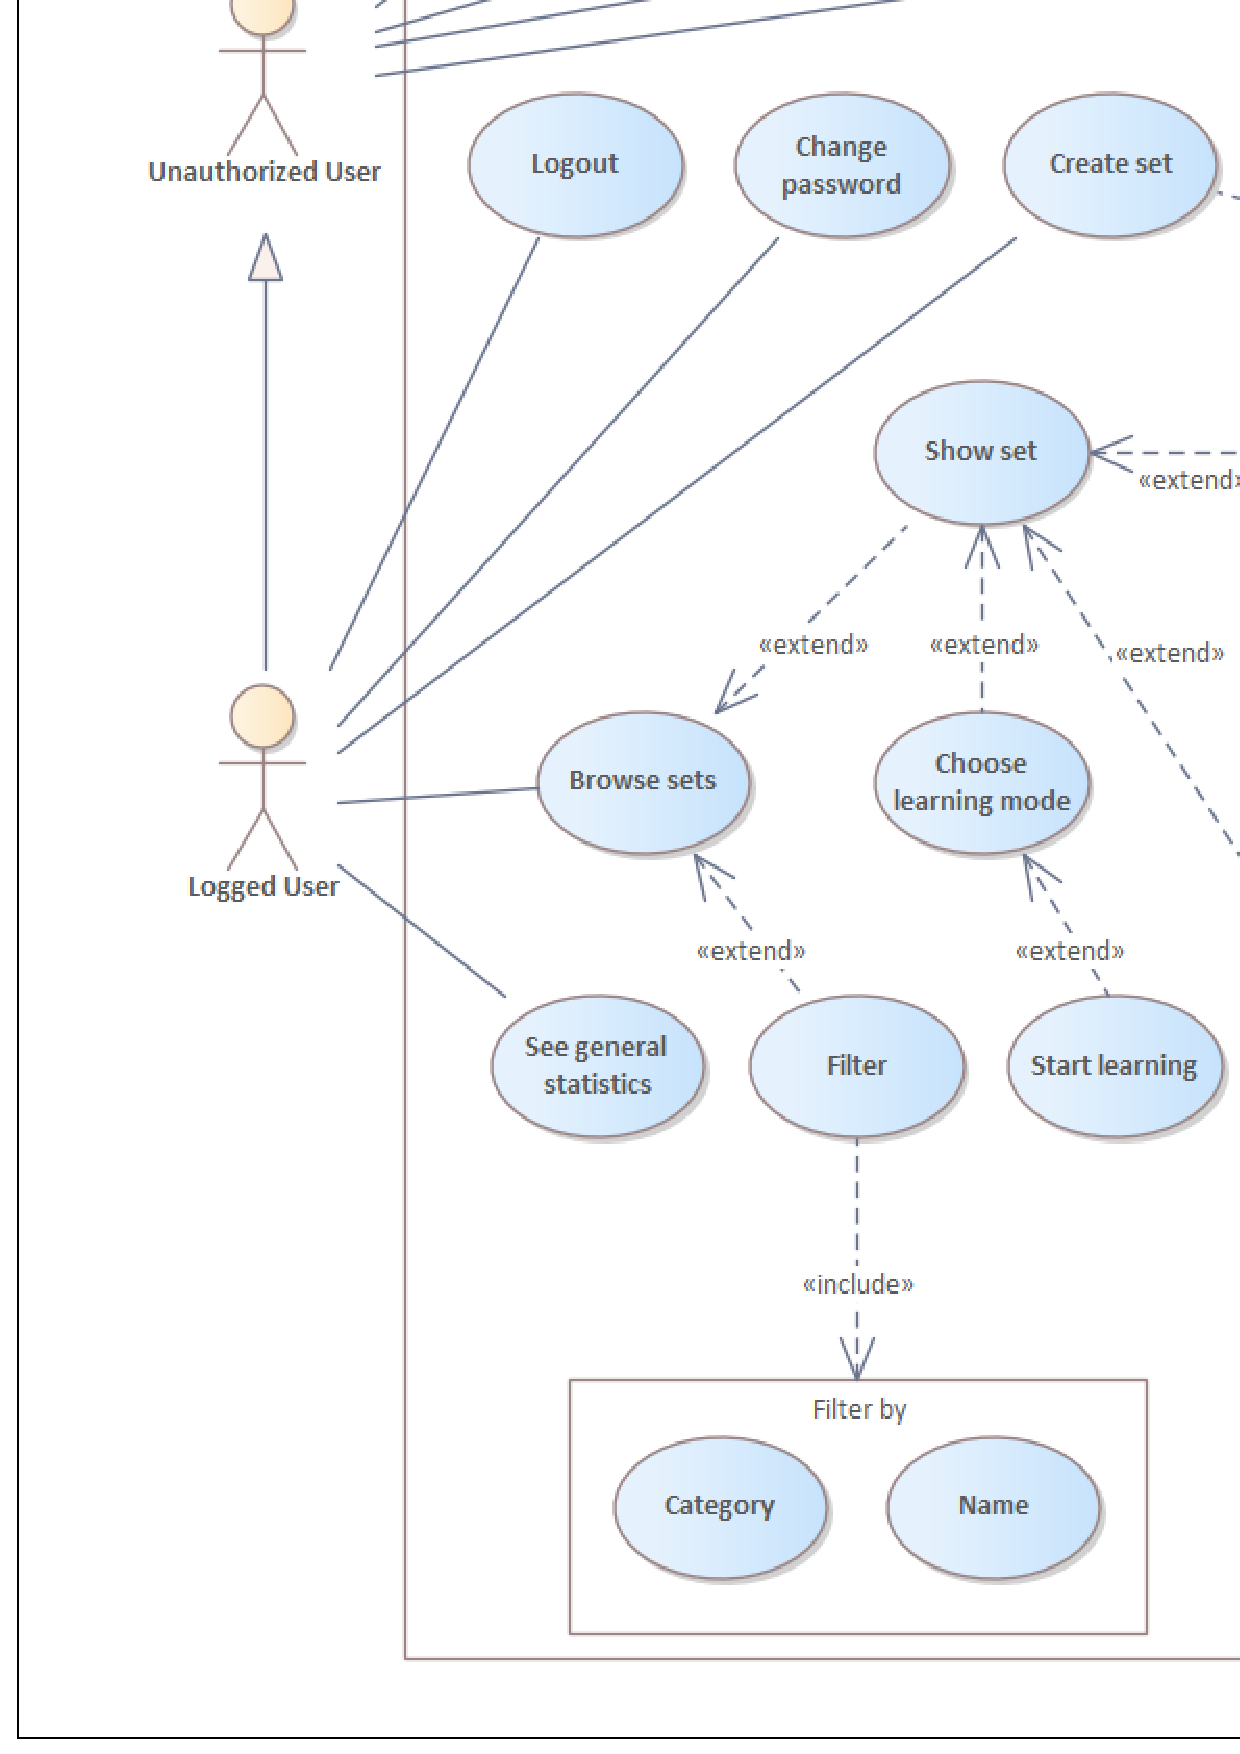
\includegraphics[width=1.32\textwidth, height=0.88\textheight]{Případy užití.png}
\caption{Diagram případů užití}
\label{fig:uc}
\end{figure}
%
%\newpage
%
%\section{Shrnutí kapitoly}
%
%V~kapitole jsme analyzovali vybraná řešení výukových aplikací flash cards, na~jejichž základě jsme specifikovali funkční i~nefunkční požadavky a~případy užití. Poznatky jsou klíčové pro~vlastní návrh implementace webové aplikace společně s~výběrem technologií a~datovým modelem.

\chapter{Výběr technologií}
\label{chap:four}

Na~základě provedené analýzy a~specifikace požadavků se tato kapitola věnuje výběru technologií, jež se použijí v~implementaci vlastní aplikace. Architektura aplikace je rozdělena na~backend a~frontend. 
%
%V podkapitolách vysvětlíme tyto části, obeznámíme se s~konkrétními, populárními technologiemi, ze~kterých vždy jednu vybereme.

\section{Backend}

Backend je kód, jenž běží na~serveru, ale klienti ho nevidí. Ovšem od~nich přijímá požadavky, zpracovává je a~obsahuje logiku pro~odesílání příslušných dat zpět klientovi. Obvykle se backendem rozumí samotný server, aplikace běžící na~serveru a~databáze pro~uchování a~uspořádání dat. S~frontendem je propojen prostřednictvím aplikačního programového rozhraní neboli API (angl.~Application Programming Interface)~\cite{codecademy}.

\subsection{Databáze}

Databáze je organizovaná kolekce strukturovaných nebo nestrukturovaných informací či dat, obvykle persistentně uložených v~počítačovém systému. Je obvykle řízena systémem správy databází neboli DBMS (angl.~Database Management System). Bezpečně manipuluje s~daty a~udržuje jejich integritu a~konzistenci. K~datům lze snadno přistupovat, spravovat je, upravovat, aktualizovat, kontrolovat a~organizovat. Databáze se běžně rozdělují na~relační SQL a~nerelační NoSQL~\cite{ordat, altex}.

\begin{itemize}
\item \textbf{Relační databáze}

Relační databáze organizují data do~strukturovaných tabulek s~řádky a~sloupci a~vytvářejí vztahy mezi nimi. Komunikaci s~databází zajišťuje Structured Querry Language, zkráceně SQL. Škálování těchto databází mezi servery pro~zajištění větší kapacity může být náročné, aby se data nenarušila. Dodržují shodu s~ACID vlastnostmi (angl.~Acid, Consistency, Integrity, Durability)~\cite{altex}.

\newpage

\item \textbf{Nerelační databáze}

Nerelační databáze ukládají data ve~formátech, jako jsou dokumenty, páry klíč-hodnota, grafové struktury nebo široké sloupce. Umožňují ukládat a~manipulovat s~nestrukturovanými nebo polostrukturovanými daty, jako je text, obrázky a~videa. Pro~větší kapacitu se dobře škálují přidáním více serverů. Ve srovnání s~relačními databázemi však neumožňují plnou podporu vlastností ACID~\cite{altex}.
\end{itemize}

V~kontextu NoSQL databází jsou nejpopulárnější systémy MongoDB (dokumentový formát), Redis (formát klíč-hodnota), Apache Cassandra (formát širokých sloupců) a~Neo4j (grafový formát)~\cite{dbengines}.

Pro~vývoj webové aplikace flash cards se musí nezbytně udržet vlastnosti ACID a~dopředu je známa její architektura. Proto se přistoupí na~použití relační SQL databáze, jejíž populární systémy jsou níže představeny.

\subsubsection*{Oracle}

Oracle je jedním z~nejpopulárnějších systémů, který nabízí vysoký počet funkcí s~vysokou škálovatelností, spolehlivostí a~robustním zabezpečením~\cite{databases}. Disponuje AI enginem pro~podporu vývojářů. Podporuje mnoho relačních i~nerelačních data modelů v~jedné databázi. Nabízí možnost databáze v~cloudu a~na~vlastním serveru. Komerční licence jsou ovšem velmi drahé. Proto se doporučuje hlavně velkým firmám nebo vládním institucím~\cite{altex, oracle}.

\subsubsection*{MySQL}

MySQL je nejpopulárnější open-source relační databázový systém, nyní pod~firmou Oracle, s~velikou komunitní podporou několik desetiletí. Disponuje jednoduchou optimalizovanou rychlostí, syntaxí a~menší komplexitou. To má ale za~následek menší robustnost v~bezpečnosti. Je navržena pro~web a~je podporována většinou cloud poskytovatelů. Doporučuje se pro~menší webové systémy nebo IoT aplikace~\cite{altex, mysql}.

%\subsubsection*{MSSQL}
%
%Microsoft SQL Server je komerční relační databázový systém primárně pro~operační systém Windows. Pro~komunikaci se používá Transact-SQL (T-SQL), což je rozšířený standardní SQL jazyk. Podobně jako Oracle je systém bohatý na~množství funkcí s~robustním zabezpečením a~spolehlivostí díky integraci s~dalšími Microsoft produkty a~nástroji. Licence jsou drahé a~doporučuje se pro~větší firmy, které pracují v~Microsoft ekosystému~\cite{databases, mssql}.
%
%\newpage
%
\subsubsection*{PostgreSQL}

PostgreSQL je open-source objektově orientovaný relační databázový systém, jenž je nejpoužívanějším vedle MySQL, s~nímž sdílí hodně společného. Nabízí ovšem více pokročilých funkcí, robustnější škálovatelnost a~integritu dat, kvůli čemuž je syntax složitější. Kompletně splňuje vlastnosti ACID. Doporučuje se pro~všechny, kteří vyžadují objektově orientované schopnosti systému či mnoho robustních funkcí a~používat plně open-source technologii~\cite{databases, postgre}. 

%Níže uvádíme silné a~slabé stránky databázového systému PostgreSQL.
%
%\begin{itemize}
%\item \textbf{Silné stránky:}
%\begin{itemize}
%\item Pokročilé funkce, jako jsou triggery, uložené procedury a~funkce pro~komplexní manipulaci s~daty a~automatizaci.
%\item Splnění ACID se~silnou zárukou integrity dat.
%\item Rozšiřitelná architektura umožňující vlastní datové typy a~funkce.
%\end{itemize}
%\item \textbf{Slabé stránky:}
%\begin{itemize}
%\item Těžší syntax ve~srovnání s~MySQL díky širší sadě funkcí.
%\item Nižší výkon oproti konkurenci.
%\end{itemize}
%\end{itemize}

\newpage

\subsection{Frameworky}

Backend frameworky tvoří podstatnou část aplikace a~nabízí různé nástroje pro~správu serverových operací a~databází. Framework je ekosystém, který pomáhá urychlit a~automatizovat kroky procesu vývoje webové aplikace. Výběr správného frameworku je klíčový a~pomůže s~rychlostí a~efektivitou vývoje samotné aplikace~\cite{radix}.

\subsubsection*{Django}

Django je open-source škálovatelný a~modifikovatelný framework na~vysoké úrovni napsán v~jazyce Python. Je rychlý a~postará se o~běžné úkoly, jako jsou autorizace uživatelů, administrace a~mapy stránek. Pomáhá vývojářům vyhnout se bezpečnostním chybám~\cite{django}. 

Je založen na~principu Don't Repeat Yourself (DRY), což pro~vývojáře znamená neopakovat kusy kódu. Řídí se design patternem Model View Controller (MVC). Díky Python funkcím splňuje CRUD vlastnosti (angl.~Create, Read, Update, Delete)~\cite{frameworks}. 

Je optimalizován pro~Search Engine Optimization (SEO) a~disponuje velkou komunitou. Doporučuje se pro~vývoj webových stránek, kde je potřeba hlavně výkon~\cite{radix}.

\subsubsection*{Laravel}

Laravel je open-source webový backend framework psaný v~PHP, který se řídí vzorem MVC. Je jedním z~nejpoužívanějších na~světě, protože většina stránek je psána právě v~PHP. Obsahuje mnoho knihoven, API podpory, databázových nástrojů jako je Object Relational Mapping (ORM), a~dokáže robustně připravit celou serverovou část aplikace. Nabízí vlastní příkazový řádek rozhraní, migraci databáze a~integraci s~mnoha databázovými systémy~\cite{radix, frameworks}. 

Disponuje expresivní a~elegantní syntaxí, což vývojářům zpříjemňuje vývoj aplikací. Ačkoli se jedná o~jeden framework, nabízí mnoho rozšíření pro~aplikace psaných čistě v~PHP nebo využívajících jiný jazyk na~jejich frontendu~\cite{laravel}.
%
%\subsubsection*{Express}
%
%Express je minimalistický a~flexibilní nadstavbou Node.js, jenž nabízí robustní set funkcí pro~webové a~mobilní aplikace. Je psán v~JavaScriptu a~díky HTTP prospěšným metodám a~middleware modulům umožňuje vytvořit robustní API rozhraní. Disponuje velkou rychlostí s~funkcemi novými i~převzatými z~Node.js~\cite{express}. 
%
%Vývojáři mohou využít Node.js pro~frontend i~backend prostředí a~Express je tedy výhodnou volbou pro~správu backendu. Umožňuje vývojářům vytvářet jednostránkové, vícestránkové, a~dokonce i~hybridní stránky~\cite{radix, frameworks}. 

\subsubsection*{Spring Boot}

Spring Boot je open-source framework, jenž usnadňuje vytváření samostatných produkčních aplikací založených na~Springu v~jazyce Java. Spring Boot aplikace vyžadují pouze minimální konfiguraci Spring prostředí~\cite{springboot, medium}. 

Díky Spring ekosystému je tento framework dobře škálovatelný, výkonný a~díky populárnímu jazyku Java i~oblíbený v~komunitě vývojářů~\cite{radix}. 

Řídí se MVC vzorem a~splňuje CRUD vlastnosti. Nabízí mnoho užitečných funkcí, jako je správa transakcí, monitorování, ukládání do~mezipaměti a~zabezpečení~\cite{frameworks}.

%Na~další straně uvádíme silné a~slabé stránky backend frameworku Spring Boot.
%
%\newpage
%
%\begin{itemize}
%\item \textbf{Silné stránky:}
%\begin{itemize}
%\item Díky autokonfiguraci se vývojář může hned zaměřit na~byznys logiku vyvíjené aplikace.
%\item Vhodný pro~vytváření architektur založených na~microservices.
%\item Integruje se s~dalšími projekty Spring, jako jsou Spring Data, Spring Security a~Spring Cloud, což usnadňuje vytváření složitých aplikací.
%\item Podpora pro~vestavěné webové servery jako Tomcat, Jetty a~Undertow. Není tedy nutno nastavovat externí server.
%\item Autokonfigurace mnoha aspektů aplikace na~základě knihoven a~závislostí zahrnutých v~projektu.
%\end{itemize}
%\item \textbf{Slabé stránky:}
%\begin{itemize}
%\item Kvůli rozsáhlosti Spring frameworku je pro~začátečníky složité se s~ním naučit.
%\item Složité přepsání a~modifikace konfigurace a~konvencí.
%\end{itemize}
%\end{itemize}
%
\section{Aplikační programové rozhraní}

Mechanismus, jenž umožňuje dvěma softwarovým komponentám vzájemně komunikovat, se nazývá aplikační programové rozhraní neboli API (angl.~Application Programming Interface)~\cite{aws}.

Rozhraním se myslí dohoda o~komunikaci mezi dvěma komponentami. Určuje, jak spolu budou komunikovat pomocí požadavků a~odpovědí, jejichž struktury jsou popsány v~API dokumentaci. Komunikace je v~tomto smyslu vykonávání operací, předávání dat a~podobně~\cite{aws}.

Aplikační programová rozhraní se používají s~protokoly, jako jsou HTML pro~API webová, XML pro~SOAP a~JSON pro~REST~\cite{mediumapi}. Význam zkratek je vysvětlen níže v~podkapitolách.
%
%Podle implementace se dají rozdělit na~několik typů. Probereme tři nejpoužívanější na~trhu.

\subsection{REST}

REpresentational State Transfer zkráceně REST funguje pomocí HTTP protokolu. Používá určité metody jako je GET, POST, PUT, DELETE a~další. Jako data formát se používá nejčastěji JavaScript Object Notation (JSON) nebo Extensible Markup Language (XML)~\cite{mediumapi}. Pokud rozhraní dodržuje REST principy, nazývá se RESTful API. Těmito principy jsou jednotné rozhraní, rozdělení na~části klient--server, bezestavovost, vrstvený systém a~volitelně další kód na~vyžádání~\cite{rest}.
%
%\begin{itemize}
%\item \textbf{Jednotné rozhraní:} Musí být umožněno klientům přistupovat ke~zdrojům a~komunikovat s~nimi konzistentním způsobem.
%\item \textbf{Klient-Server:} Aplikace musí být rozdělena na~části klient a~server, což umožňuje nezávislý vývoj každé z~nich.
%\item \textbf{Bezestavovost:} Každá interakce mezi klientem a~serverem je nezávislá. Server neukládá žádný kontext klienta mezi požadavky.
%\item \textbf{Ukládat do mezipaměti:} Možnost ukládat odpovědi do~mezipaměti, aby se mohly použít znovu pro~stejné dotazy.
%\item \textbf{Vrstvený systém:} Vrstvená architektura umožňuje připojení více bodů. Klient nemůže rozlišit, zda je připojen ke~koncovému serveru nebo s~prostředníkem.
%\item \textbf{Kód na vyžádání (volitelné):} Rozšíření funkčnosti pro~přenos spustitelného kódu pro~spuštění na~straně klienta.
%\end{itemize}

REST je efektivní, výkonný, škálovatelný, jednoduchý na~údržbu i~integraci a~flexibilní z~hlediska datových formátů~\cite{mediumapi, milan}.

Příkladem komunikace může být API na~sociální platformě pro~povolení načítání uživatelských příspěvků aplikacemi třetích stran~\cite{milan}.

\subsection{SOAP}

Simple Object Access Protocol zkráceně SOAP je architektura umožňující přenos dat se~silnou a~robustní bezpečnostní strukturou. Ke~komunikaci se používá XML data formát a~API funguje primárně pomocí HTTP nebo SMTP protokolu, ale i~dalších. Používá se hlavně v~systémech, kde je bezpečnost komunikace na~prvním místě~\cite{mediumapi, milan}.

Je platformově nezávislý, komplexnější a~bezpečnější než REST. Disponuje silným zabezpečením a~transakčními schopnostmi, robustním zpracováním chyb a~správou výjimek, ale malou flexibilitou a~výkonností především kvůli XML formátu~\cite{dev}.

Příkladem použití může být přenos prostředků mezi účty u~finančních institucí využívajících zabezpečené transakční operace~\cite{milan}.

\newpage

\subsection{GraphQL}

GraphQL je nejen architektura, ale i~dotazovací jazyk umožňující klientům ptát se na~specifická data, jež přesně potřebují. Funguje pomocí HTTP protokolu. Výsledkem je efektivnější komunikace a~rychlejší odpovědi. Společnost Meta vyvinula toto API, aby se přesná data doručila miliardám uživatelů. Díky flexibilitě a~účinnosti je výbornou volbou pro~aplikace s~komplexními datovými požadavky~\cite{dev}. 

Je platformově nezávislý a~silně typovaný, což zajišťuje konzistentní a~kompatibilní data mezi klientem a~serverem. Disponuje pouze jedním koncovým bodem, díky čemuž je efektivnější než REST, a~ptá se přesně na~to, co si klient přeje. Podporuje také dotazy typu mutace či předplatné~\cite{dev}.

Příkladem použití může být efektivní načítání produkčních dat v~mobilních aplikacích včetně pouze polí, která mají být zobrazena~\cite{milan}.

\section{Frontend}

Frontend je klientská část aplikace, s~níž klient interaguje. Hlavní jazyky použité pro~tuto část jsou HTML, CSS a~JavaScript. Jelikož je požadováno, aby webová aplikace byla responzivní a~uměla různé funkce, bude použit JavaScript jako jazyk frontendu aplikace, který ulehčí její tvorbu. Frontendových frameworků existuje na~trhu mnoho, probrány jsou tři nejpoužívanější, a~to React, Vue.js a~Angular~\cite{frontend}.

\subsection{React}

React je nejpopulárnější open-source knihovna pro~JavaScript k~tvorbě frontendu webových stránek. Společnost Meta ho původně vytvořila pro~řešení problémů spojených s~dynamickými a~komplexními uživatelskými rozhraními. React využívá virtuální Document Object Model (DOM), což umožňuje vývojářům efektivně aktualizovat pouze části uživatelského rozhraní, jež se změnily, a~přitom nenačítat celou stránku znovu~\cite{roadmap, react}.

Výhodou je využití znovupoužitelných komponent, konzistentní výkon díky virtuální DOM, pokročilé nástroje a~množství vylepšujících balíčků. Knihovna je doporučena hlavně pro~tvorbu Single Page aplikací díky virtuálnímu DOM konceptu. Pro~začátečníky může být ovšem obtížné se v~knihovně zorientovat kvůli komplexitě JavaScript XML (JSX) a~React hooks~\cite{simform}.

\subsection{Vue.js}

Vue.js je open-source framework, který vznikl v~roce 2014 ve~snaze zkombinovat nejlepší části Angular s~jednoduchostí a~flexibilitou Reactu. Je znám díky své progresivitě, což vývojářům umožňuje postupně se adaptovat na~jeho funkce a~kompletně nepřepisovat existující projekt~\cite{roadmap, vue}. Podobně jako React disponuje virtuálním DOM konceptem pro~znovupoužití komponent na~stránce pro~zvýšení efektivity a~výkonu~\cite{wad}.

Výhodou je jednoduchá syntax, detailní dokumentace a~flexibilita. Ovšem komponenty mohou být nestabilní. Jelikož je Vue.js celkem novým produktem, obklopuje ho malá komunita, především z~Asie. Dokumentace některých balíčků neexistuje v~angličtině~\cite{simform, wad}.
%
%\newpage

\subsection{Angular}

Angular se v~roce 2010 představil jako AngularJS pod~firmou Google s~možností obousměrné vazby dat a~vkládání závislostí. V~roce 2016 Google celý framework přepsal z~důvodu komplexity a~nazval ho Angular. Obousměrná vazba dat znamená synchronizaci mezi modelem a~pohledem (angl.~Model and View) v~reálném čase. Podobně jako React nebo Vue.js disponuje znovupoužitelností komponent díky vkládání závislostí (angl.~dependency injection) pro~DOM~\cite{roadmap, wad}.

Výhodou je velké množství funkcí i~balíčků a~zmíněná obousměrná vazba dat. Ovšem i~přes detailní dokumentaci je kvůli své komplexitě složitý pro~začátečníky. Používají ho hlavně velké společnosti~\cite{simform, wad}.

\section{Použité technologie}

Kapitola se zabývala technologiemi zahrnující backend, rozdělený na~databáze a~frameworky, frontend a~aplikační programové rozhraní pro~komunikaci mezi klientskou a~serverovou částí.% V~podkapitolách jsme u~použitých nástrojů zdůvodnili jejich výběr pro~webovou aplikaci flash cards.

%V~budoucí bakalářské práci bychom se zabývali výběrem vhodného server hostingu pro~nasazení aplikace, pokud by nebylo možné aplikaci nasadit na~server poskytnutý FEL ČVUT.

V~následující tabulce~\ref{tab:techshr} jsou vypsány použité technologie se~shrnutými důvody výběru pro~vlastní implementaci aplikace.

\begin{table}[H]
\caption{Vybrané použité technologie}
\begin{tabular}{| >{\centering\arraybackslash}m{3cm} | >{\centering\arraybackslash}m{4cm} | >{\centering\arraybackslash}m{5cm} |}
\hline
 & \textbf{Vybraná technologie} & \textbf{Důvod výběru} \\ \hline
\textbf{Databáze} & PostgreSQL & Pokročilé funkce, splnění ACID a~předešlá zkušenost \\ \hline
\textbf{Backend framework} & Spring Boot & Funkce, MVC, splnění CRUD, Java a~předešlá zkušenost \\ \hline
\textbf{API} & REST & Funkce, jednoduchost a~předešlá zkušenost \\ \hline
\textbf{Frontend framework} & React & Popularita, doporučení, funkce a~výkon \\ \hline
\end{tabular}
\label{tab:techshr}
\end{table}

\chapter{Návrh implementace}

Po~detailní analýze a~výběru technologií je navrhnuta samotná aplikace. Kapitola je rozvrhnuta do~několika podkapitol, které se blíže věnují jednotlivým částem, jež obecně návrh obsahuje. Zabývá se datovým modelem, komponentami aplikace, sekvencemi, architekturou a~v~neposlední řadě návrhem testování. Obrázky diagramů byly vytvořeny v~nástroji Enterprise Architect~15~\cite{ea}.

\section{Datový model}
\label{sec:fiveone}

Webová aplikace obecně potřebuje persistentní uložení dat v~databázi na~serveru. Implementace musí umožňovat ukládat uživatelská data včetně všech vytvořených setů.

Diagram datového modelu \ref{fig:dm} na~další straně obsahuje entity, jež jsou potřebné k~implementaci a~persistentnímu ukládání dat. Tabulky obsahují primární klíče a~propojují se cizími klíči.

\newpage

\begin{figure}[H]
\includegraphics[width=1.4\textwidth, height=0.98\textheight, center]{Datový model.png}
\caption{Datový model aplikace}
\label{fig:dm}
\end{figure}

\section{Komponenty}
\label{sec:fivetwo}

Komponenty aplikace flash cards se dají rozdělit do~tří vrstev. Prezentační vrstva s~Reactem je propojena pomocí REST API s~aplikační vrstvou s~logikou samotné aplikace, jež je dále propojena ORM s~datovou vrstvou s~PostgreSQL databází.

V~této podkapitole se řeší komponenty aplikace, které jsou nejvíce rozmanité v~aplikační vrstvě. Na diagramu~\ref{fig:cd} na~další straně je backend rozdělen do~balíčků Controller, Service, Repository a~Model.

Komponenty v~Controller balíčku zpracovávají komunikaci uživatele s~aplikací pomocí REST API. Balíček Service obsahuje byznys logiku aplikace. Repository balíček zajišťuje komunikaci s~databází a~komponenty v~balíčku Model reprezentují datové entity~\cite{csrm}.

\newpage

\begin{figure}[H]
\includegraphics[width=1.4\textwidth, height=1.72\textwidth, center]{Diagram komponent.png}
\caption{Diagram komponent aplikace}
\label{fig:cd}
\end{figure}

\newpage

\section{Sekvence}
\label{sec:fivethree}

Sekvence konkrétních úkonů či mechanismů aplikace pomáhají bližšímu porozumění jejího fungování. Diagram~\ref{fig:sd} níže ukazuje sekvenci používání při~přihlášení uživatele do~aplikace.

\begin{figure}[H]
\centering
\includegraphics[width=1.17\textwidth, height=0.83\textheight]{Sekvenční diagram Přihlášení.png}
\caption{Sekvenční diagram přihlášení uživatele}
\label{fig:sd}
\end{figure}

\newpage

\section{Architektura}

Pro aplikaci bylo zvoleno rozdělení na~část klientskou a~serverovou. Části spolu komunikují pomocí REST API s~datovým formátem JSON, jak bylo zmíněno v~kapitole \ref{chap:four}.

Architektury software se běžně rozdělují na~dvě struktury, a~to monolitické architektury a~mikroslužby (angl.~microservices)~\cite{monomicro}.

Software využívající monolitickou architekturu je navržen jako jeden celek. Každá součást aplikace je těsně integrována a~celá aplikace je nasazena jako jeden blok. Tato architektura se volí při~menších projektech, které nejsou příliš komplexní, protože je jednodušší na~vývoj~\cite{monomicro}.

Aplikace využívající mikroslužby je rozdělena do~malých, nezávislých služeb, jež spolu spolupracují. Každá část je odpovědná za~konkrétní funkčnost aplikace a~může být nezávisle vyvíjena na~částech ostatních. Tato architektura se doporučuje pro~vývoj komplexních a~velkých projektů~\cite{monomicro}.

Pro~implementaci aplikace bude využita monolitická architektura z~důvodu velikosti práce, konkrétně třívrstvá architektura klientské a~serverové části rozdělená na~prezentační, aplikační a~datovou vrstvu. Na~diagramu \ref{fig:dd} níže je vyobrazeno nasazení aplikace.

\begin{figure}[H]
\centering
\includegraphics[width=1\textwidth, height=0.3\textheight]{Diagram nasazení.png}
\caption{Diagram nasazení aplikace}
\label{fig:dd}
\end{figure}

\newpage

\section{Návrh obrazovek UI}

Důležitým aspektem návrhu webové aplikace jsou samotné obrazovky uživatelského rozhraní. Jsou demonstrovány hlavní dvě části, a~to přihlášení při~prvotním načtení stránky a~sety flash karet jako domovskou stránku po~přihlášení uživatele. Návrhy na~obrázcích \ref{fig:login} a~ \ref{fig:sets} níže byly vytvořeny v~nástroji Figma~\cite{figma}.

\begin{figure}[H]
\centering
\includegraphics[width=1.1\textwidth, height=0.36\textheight]{Login.png}
\caption{Návrh přihlašovací obrazovky}
\label{fig:login}
\end{figure}

\begin{figure}[H]
\centering
\includegraphics[width=1.1\textwidth, height=0.36\textheight]{MainMenu.png}
\caption{Návrh obrazovky hlavního menu se~sety karet}
\label{fig:sets}
\end{figure}

\newpage

\section{Návrh REST API}

Ke~komunikaci backendu a~frontendu bude použito RESTful API. Pomocí generátoru specifikace OpenAPI níže na~obrázcích \ref{fig:authapi} a~\ref{fig:setsapi} je představen návrh několika základních koncových bodů ohledně autorizace a~kolekcí karet.

Koncové body \emph{/auth/delete-account/\{userId\}}, \emph{/auth/get-all-users}, \emph{/card-sets/get-all} a~\emph{/card-sets-get-cards} budou dostupné pouze pro~administrátora. Koncový bod \emph{/card-sets/get-sets} využije stránkování pro~efektivnější práci s~databází a~zároveň zamezí přetížení klientské strany nadměrným množstvím kolekcí karet načtených najednou.

Skutečné koncové body použité v~aplikaci generované rozhraním OpenAPI jsou k~dispozici v~seznamu odkazů.

\begin{figure}[H]
\centering
\begin{subfigure}[t]{0.49\textwidth}
  \centering
  \includegraphics[width=1.1\linewidth, height=0.6\textheight]{auth.png}
  \caption{Návrh autorizačních endpointů}
  \label{fig:authapi}
\end{subfigure}
\hfill
\begin{subfigure}[t]{0.49\textwidth}
  \centering
  \includegraphics[width=1.1\linewidth, height=0.6\textheight]{sets.png}
  \caption{Návrh endpointů kolekcí karet}
  \label{fig:setsapi}
\end{subfigure}
\caption{Návrh základních endpointů}
\label{fig:apis}
\end{figure}

\newpage

\section{Návrh testování}
\label{sec:fiveseven}

K~implementacím aplikací vždy patří jejich testování. Existuje několik typů testů, které jsou vhodné pro~různé části aplikace. Níže je navrženo několik druhů testování.

\subsection{Jednotkové testy}

Jednotkové testy jsou potřebné pro~testování jednotlivých funkcí a~metod programu. Metody na~serverové části aplikace budou testovány těmito testy, jež budou využívat frameworky JUnit a~Mockito.

\subsection{Integrační testy}

Integrační testy testují, jak~spolu jednotlivé metody spolupracují v~různých částech systému. Jsou rozsáhlejší velikosti a~ budou pro~ně vytvořeny testovací scénáře. Budou využity pro~testování komunikace backendu s~databází.

\subsection{Procesní testy}

Procesní testy simulují chování uživatele a~testují celý proces, který je potřeba pomocí diagramu vyjádřit. Mohou být rozsáhlé velikosti a~vždy pro~ně budou vytvořeny testovací scénáře. Těmito testy bude testována námi vytvořená sekvence a~další procesy v~případech užití.

\subsection{Uživatelské testy}

Uživatelské testy budou testovat chování aplikace na~úrovni reálných uživatelů. Zapojí se několik uživatelů pro~zjištění, zda se webová aplikace používá intuitivně a~zobrazuje se i~funguje správně na~mobilních či počítačových zařízeních. Uživatelé budou zprostředkovávat zpětnou vazbu pro~opravy a~vylepšení aplikace prostřednictvím dotazníků.

%\section{Shrnutí kapitoly}
%
%V~kapitole jsme navrhli implementaci aplikace flashcards, a~to datový model databáze, komponenty i~sekvence aplikace a~architekturu programu. Poté jsme navrhli i~typy testů, jež budou potřeba pro~otestování aplikace a~její nejrůznější opravy.
%
\chapter{Implementace aplikace}

V~této kapitole je probrána samotná implementace webové aplikace. V~podkapitolách se řeší použité nástroje k~implementaci obou částí. Poté je popsána implementace backendu i~frontendu a~jednotlivé stránky. Implementace je seřazena chronologicky až na~menší výjimky. Backend i~frontend projekty byly implementovány současně.

K~verzování kódu byla využita služba GitHub a~nástroj Git, což je distribuovaný systém pro~správu verzí. Lépe se dají sledovat změny, spolupracovat s~lidmi a~spravovat různé verze kódu~\cite{git}. V~seznamu odkazů se nachází GitHub repozitáře pro~frontend a~backend.

\section{Nástroje pro~backend}
\label{sec:sixone}

Pro~implementaci backend Spring aplikace díky autorovy předešlé zkušenosti bylo použito vývojové prostředí JetBrains IntelliJ IDEA Ultimate, což je velmi populární IDE hlavně pro~jazyky Java a~Kotlin. Díky podpoře frameworků a~pluginů IDE bohatě vystačilo pro~celou Spring aplikaci včetně využití Hibernate, Maven, a~dalších nástrojů~\cite{idea}.

Díky verzi Ultimate bylo využito pokročilé podpory pro~frameworky a~pluginy. Velkým přínosem verze je práce a~propojení s~PostgreSQL databází, kde jsou dostupné všechny entity i~query konzole. Také je snažší vytvořit Docker kontejner pro~sestavení a~nasazení backendu ke~cloud poskytovateli a~využívat verzování pomocí Git~\cite{ideaf}.

Pro~testování API endpointů ještě před~propojením s~frontendem byl využit testovací nástroj Postman, který je velmi populární a~disponuje skvělým laděním endpointů a~generováním dokumentace~\cite{postman}.

K~sestavení backend části aplikace byl použit Apache Maven. Tento nástroj je velmi důležitou součástí projektu a~všech závislostí. Vše je řízeno z~\emph{pom.xml} souboru~\cite{maven}. Pro~nasazení na~produkční server u~poskytovatele se ještě využil Docker kontejner, jenž umožňuje konzistenci běhu backendu~\cite{docker}.

Verze nejdůležitějších použitých nástrojů jsou Java JDK~21, Spring Boot 3.5.0-SNAPSHOT, PostgreSQL~17.4 a~Apache Maven~3.9.9.

\section{Nástroje pro~frontend}

Pro~implementaci frontend React webové aplikace díky autorovy předešlé zkušenosti bylo použito vývojové prostředí Visual Studio Code. S~Reactem se zde lépe pracuje. VS Code je open-source IDE od~Microsoft, které je velmi flexibilní. V~základu je lehké, ale dá se rozšířit mnoha pluginy včetně verzování pomocí Gitu a~pomocníků pro~práci s~React aplikací~\cite{vscode}.

Jelikož vytvoření projektu pomocí \emph{create-react-app} od~Reactu je zastaralé, byl použit nynější framework Next.js od~Vercel, jenž je na~Reactu postaven. Rozšiřuje možnosti o~serverové funkce, generování stránky na~serveru, rychlejší načítání stránek, optimalizaci pro~SEO, a~další. K~vytvoření projektu se použil příkaz \emph{create-next-app}, což zařídilo jeho základní konfiguraci~\cite{nextjs}.

Kvůli tomu, že je framework pro~autora novinkou, postupovalo se podle doporučených nastavení. Ta zahrnovala využití Node.js pro~JavaScript, VS Code jako IDE, ESLint pluginu ke~kontrole kvality kódu pro~JavaScript i~TypeScript, a~samotného TypeScriptu, což je nadstavba JavaScriptu se~statickým typováním. ESLint dokáže najít chyby, nekonzistence i~problémy v~kódu již při~jeho psaní a~TypeScript umožňuje definovat typy proměnných, funkcí i~objektů pro~odhalení chyb již při~kompilaci programu~\cite{eslint, typescript}.

K~sestavení React aplikace na~serveru u~poskytovatele se využívá příkaz \emph{next build} a~ke~startu příkaz \emph{next start}. Testování probíhalo ve~webovém prohlížeči Brave, který je založen na~Chromiu.

Verze nejdůležitějších použitých nástrojů jsou Node.js~22.14.0, Next.js~15.3.0 a~React~19.1.0.

\section{Implementace databáze a~backendu}
\label{sec:sixthree}

Implementace je rozdělena chronologicky za~sebou. Je popsáno, co a~jak bylo provedeno a~kde nastaly problémy. Nakonec jsou zmíněny finální změny.

\subsection{Základní konfigurace projektu}

Díky autorovým předešlým zkušenostem byla prvotní konfigurace projektu jednoduchá. Byl vytvořen Spring Boot projekt v~IntelliJ IDEA a~přidány nutné Maven závislosti. K~balíčkům zmíněných v~podkapitole \ref{sec:fivetwo} byly přidány ještě balíčky \emph{config, dto} a~\emph{mapper}. Byly přidány \emph{resources}, které drží důležité proměnné a~nastavení Spring aplikace a~SQL příkazy migrací dat pomocí Liquibase.

V~balíčku \emph{config} se nachází Spring konfigurátor logů v~aplikaci, jenž zaznamenává podstatné události za~běhu aplikace. V~balíčku \emph{controller/interceptors} byla přidána strategie loggování, jež se zaznamenává do~příslušného souboru.

V~případě chyby jsou využity standardní výjimky Javy, které jsou zaznamenávány do~souboru, a~se~zprávami vráceny jako odpověď na~požadavek frontendu s~kódem 400 (Bad Request).
\newpage

Díky navrhnutému datovému modelu v~podkapitole~\ref{sec:fiveone} bylo vytvoření entit v~balíčku \emph{model} jednoduché. Spring a~IDE umožnily automatické vytvoření repositories pro~všechny entity. Také byly automaticky vytvořeny dto a~mappery pro~jednotlivé entity, které byly na~začátku a~postupem času měněny podle potřeb. Dto a~mappery jsou důležité pro~přenos pouze požadovaných informací a~nevydání entity API.

\subsection{Databáze}

Propojení s~databází proběhlo bez~problémů. Po~jejím vytvoření byl použit nástroj Liquibase, jenž pro~entity z~balíčku \emph{model} vytvořil SQL skript, který přidal jednotlivé entity i~jejich relace do~databáze. Jediná tabulka \emph{favourite\_sets} přítomná v~databázi není v~modelu z~důvodu využití relace ManyToMany mezi dvěma entitami a~použití Hibernate.

Pro~přidání a~úpravy entit byly využity další SQL skripty. Údaje k~připojení k~databázi jsou uloženy v~\emph{application.yml}, ovšem konkrétní hodnoty jsou skryty v~\emph{.env} souboru, který není viditelný v~GitHub repozitáři.

\subsection{Zabezpečení backendu}

Zabezpečení backendu je nedílnou součástí projektu. Neověřený uživatel nesmí mít přístup k~částem aplikace, kde se požaduje JWT token a~v~některých instancích také jeho role jako admin. Zabezpečení se nachází v~balíčku \emph{security}, jenž se dá rozdělit na~konfiguraci zabezpečení, konfiguraci JWT, odpovědí a~ovladače pro~OAuth2 Google uživatele.

Orientace v~zabezpečení byla pro~autora těžší, a~proto byl využit a~modifikován kód pro~tyto účely od~GitHub uživatele \emph{eugenp} a~návod na~stránce \emph{baeldung}~\cite{baeldungspring}. Odkazy na~všechny použité moduly v~projektu jsou k~dispozici v~seznamu odkazů.

Konfigurace zabezpečení byla první velkou překážkou implementace. Bylo nutné přidat první balíček \emph{userdetails} do~již existujícího \emph{service} balíčku pro~správnou funkčnost konfigurace zabezpečení a~logiku přihlášení, odhlášení i~registrace. Také byl vytvořen první controller pro~práci s~uživateli. Autorizační JWT token byl ukládán do~cookies. Ovšem kvůli využití různých domén frontendu a~backendu bylo nutné záležitost vyřešit pomocí headers, jak bylo v~návodu. Situace je blíže specifikována v~podkapitole~\ref{sec:sixsix} níže, protože pro~autora byla dalším velkým problémem.

Byl vybrán JWT (JSON Web Token) pro~autorizaci především kvůli jeho použití v~návodech, využití u~bezestavových aplikací a~integrace se~Spring Security pro~zabezpečení REST API. Klíčovým procesem generování tokenů je použití podpisu pro~zaručení pravosti~\cite{baeldungspring}.

Po~vyřízení ověření uživatelů přihlášených či zaregistrovaných standardní cestou s použitím e-mailu a~hesla, se přešlo na~implementaci OAuth2 autorizace uživatelů s Google přihlášením. Pro~OAuth2 byl využit další návod o~dvou částech z~článku na~stránce Medium~\cite{oauth1, oauth2}.

Bylo nutné v~Google API konzoli vytvořit \emph{Authorized redirect URI} pro~přesměrování uživatele na~přihlašovací stránku Google a~také zkopírování \emph{Client ID} a~\emph{Client secret} do~skrytého \emph{.env} souboru pro~následné využití v~aplikaci. Také byl vytvořen další balíček \emph{oauth2} v~\emph{service}, kde se nachází logika přihlášení, odhlášení i~registrace pomocí účtu Google. S OAuth2 uživatelem je po~přihlášení zacházeno jako s uživatelem klasickým, je mu generován JWT token a~je přesměrován na~příslušnou stránku frontendu.

OAuth 2.0 je standard navržený tak, aby umožnil webu nebo aplikaci přístup ke~zdrojům hostovaným jinými webovými aplikacemi jménem uživatele~\cite{oauth1}. Použití OAuth2 pro~přihlášení pomocí Google účtu je komfortní cestou v~implementaci.

\subsection{Uživatelé}

Po dokončeném ověření uživatelů společně s~registrací a~přihlášení byla implementována možnost upravit si údaje účtu nebo smazat účet. Také byl přidán vzor Builder pro~vytvoření uživatele, protože se vytváří na~více místech (standardní registrace nebo OAuth2) a s~jinými specifikacemi.

Dále se se~zaregistrováním uživatele vytvoří jeho globální uživatelské statistiky napříč celou aplikací, kde se jednotlivé statistiky zvyšují při~vykonání určitých akcí. Příkladem může být vytvoření kolekce nebo karty. 

Při~registraci se uživateli pošle uvítací zpráva na~uvedený e-mail. Nutností bylo přidání informace o~automatickém e-mailovém účtu do \emph{.env} souboru pro~využití ve~Spring aplikaci.

Když uživatel zapomene heslo, může si ho obnovit. K~tomuto je na~backendu implementována logika generace a~ověření časově omezených tokenů. Na~uvedený e-mail se token pošle a~po zadání se ověří. Pokud je správný, uživatel si může zvolit nové heslo.

\subsection{Kolekce a~karty}

Před~vytvořením samotných kolekcí bylo nutné implementovat získávání filtrovaných kolekcí se~stránkováním. K~filtraci je využit vzor Chain of responsibility, protože je vždy proces filtrování stejný, jen použité filtry se mohou lišit. Každý filtr má své opodstatnění. Stránkování je vyřešeno pomocí \emph{Pageable} a~\emph{PageRequest} od~Spring Domain.

Poté byly přidány CRUD operace pro~kolekce i~karty. Při~prvním navštívení kolekce se vytvoří její statistiky pro~daného uživatele. Tyto statistiky se zvyšují učením se dané kolekce.

V~pozdějším vývoji bylo umožněno uživateli přidávat obrázky ke~kartám s~tím, že k~jedné kartě lze přidat jen jeden obrázek. Autor si může měnit viditelnost své kolekce ostatním uživatelům, což znamená nastavení soukromé nebo veřejné. Uživatel si může označit jakoukoliv kolekci za~oblíbenou.

\newpage

U~kolekce byla přidána možnost vytvoření její kopie, pokud daný uživatel není autorem této kolekce. Byla implementována možnost změnit si pořadí karet v~kolekci. Těmito funkcemi byl nahrazen funkční požadavek \emph{FR10 -- Formátování textu flash karet}, který není splněn z~důvodu našeho přesvědčení, že není potřebný k~tvorbě karet.

\subsection{Finální úpravy}

Do~finálních úprav se zahrnuje implementace CRUD operací pro~uživatele s~rolí admin, což je u~endpointů ověřováno zabezpečovacím filtrem. Ti mají přístup k~uživatelům, kolekcím i~kartám.

Kvůli využití různých domén frontendu a~backendu je v~balíčku \emph{controller/config} implementován konfigurátor CORS (Cross-origin resource sharing), což je mechanismus umožňující sdílení zdrojů na~jiné doméně. Dále byly využity headers pro~JWT tokeny, což je blíže upřesněno v~podkapitole~\ref{sec:sixsix}.

\section{Implementace frontendu}

Podobně jako u~backendu je implementace rozdělena chronologicky za~sebou. Podkapitola se zabývá všemi stránkami v~projektu, pomocnými soubory a~také problémy, se~kterými se autor potýkal. Provázané funkce s~backendem jsou pouze shrnuty, protože jsou zmíněny v~podkapitole~\ref{sec:sixthree}.

V~modulu \emph{public} se nachází použité obrázky a~v~modulu \emph{src} se nachází middleware, jenž je zmíněn později. V~\emph{src/app} se nachází stránky projektu a~v~kořenovém repozitáři konfigurační soubory.

Kvůli různým doménám frontendu a~backendu byly místo serverových cookies použity ty v~prohlížeči. Více informací je v~podkapitole~\ref{sec:sixsix}. Pro~uchování dat o~uživateli, aby pokaždé frontend nemusel žádat backend o~informace, je použito \emph{sessionStorage} v~prohlížeči.

\subsection{Domovská stránka, registrace a~přihlášení}

Každá stránka se skládá ze~záhlaví, hlavního obsahu a~zápatí. V~záhlaví je krátký nápis a~navigační panel. Tento panel se mění podle stavu uživatele, zda je přihlášený či ne. V~zápatí se nachází krátké prohlášení a~odkazy na~dotazníky, o~kterých píšeme později.

Byla vytvořena domovská stránka s~uvítáním a~stejným obsahem jako na~přihlašovací stránce. Uživatel se může přihlásit nebo odkázat na~stránku registrace. Později se na~stránku přidal další obsah. U~registračního formuláře je postup prakticky stejný jako u~přihlášení.

\subsection{Uživatelský účet, obnova hesla a~OAuth2}

Po~úspěšném ověření uživatele klasickou cestou byla přidána stránka uživatelského účtu, kde je možné upravit si údaje (uživatelské jméno, e-mail a~heslo), smazat si účet a~podívat se na~své globální statistiky.

Byla přidána stránka s~obnovou zapomenutého hesla, kde po zadání e-mailu a~poté ověřovacího kódu poslaného na~uvedený e-mail je možné zvolit si nové heslo k~účtu. Poté je uživatel přesměrován na~přihlašovací stránku. Odkaz byl přidán do~přihlašovacího formuláře.

Byla implementována možnost přihlásit se pomocí Google účtu. Tlačítko s~přesměrováním bylo přidáno do~přihlašovacího i~registračního formuláře.

\subsection{Procházení kolekcí a~karet}

Dřívější prázdnou stránku kolekcí byla vylepšena o~uvítací nápis, filtry vyhledávání a~pole kolekcí karet s~názvem, kategorií, autorem a~datumem vytvoření. Dále jsou dostupná tlačítka se~stránkováním a~tlačítko pro~vytvoření kolekce.

Filtry obsahují přepínače pro~autorské nebo oblíbené kolekce, vyhledávací pole podle názvu kolekcí, výběr kategorie, řazení vyhledaných výsledků a~tlačítko na~obnovu filtrů. Kliknutí na~kolekci uživatele přesměruje na~stránku kolekce. Tlačítko vytvoření kolekce otevře modální okno, kde je uživateli umožněno vlastní kolekci vytvořit a~po~úspěšném vytvoření je přesměrován na~stránku kolekce.

Stránka konkrétní kolekce dovolí autorovi ji upravit nebo smazat. Tlačítkem může přidávat nové karty s~otázkami a~odpověďmi, jež může také upravovat a~mazat. Pořadí karet v~kolekci může uživatel měnit pomocí příslušných tlačítek se~šipkami. Tlačítky se mohou kromě karet zobrazit statistiky uživatele nebo výukové módy s~popisky.

Modální okno s~přidáním nové karty je podobné jako okno s~výtvorem kolekce. Po~vytvoření se karta přidá na~konec pole karet. Ke~každé kartě je možné přidat jeden obrázek, který se přidá k~otázce. K~jednomu uživatelskému účtu je dovoleno přidat maximálně čtyři obrázky z~důvodu velikosti databáze.

Uživatel, jenž není autor, si může kolekci celou zkopírovat. Také může kolekci i~autora pomocí dotazníku nahlásit.

\subsection{Výukové režimy}

Mezi výukové režimy patří klasická metoda výuky, výběr z~více možností a~výběru pravda/nepravda. U~všech režimů je možné zopakovat si kolekci po~její celé výuce. Pokud prohlížeč funkci umožňuje, je uživatel upozorněn o~ztrátě postupu v~případě odchodu z~výukového režimu.

Klasická metoda spočívá ve~výuce každé karty kolekce jednu po~druhé. Na~začátku je volba zamíchání karet. Uživatel u~každé zvolí, jestli odpověď zná či ne. Pokud uživatel označí, že nezná odpověď na~otázku, je karta zařazena do~pole takto označených karet, které je možné na~konci výuky zopakovat.

Výběr z~více možností začíná výběrem, zda chce uživatel vybírat z~otázek nebo odpovědí. Poté se celá kolekce zamíchá a~volí se mezi čtyřmi možnostmi k~dané otázce či odpovědi.

Poslední režim spočívá v~tom, jestli je daná odpověď na~otázku pravdivá či ne. Podobně jako u~režimu výběru z~více možností je možné si na~začátku zvolit vybírání pravdivosti otázek nebo odpovědí. 

\subsection{Rozdělení frontendu do~částí}

Mimo již zmíněné soubory stránek bylo implementováno několik dalších částí, a~to kontext, vlastní React hooks (háčky) a~komponenty, jež je dělen na~TSX (TypeScript Execute) elementy, pomocné funkce a~API dotazy. Také je zmíněn middleware.

Byl přidán autorizační kontext, což je rodičovská komponenta, jež umožňuje použití jejího obsahu ve~všech jejích potomcích. Usnadňuje práci s~předáváním props nebo parametrů~\cite{context}. V~konkrétním případě pomáhá s~prací s~uživatelskými daty. Každá stránka tato data využívá a~některé se podle toho chovají.

React hooks jsou velmi silnou součástí Reactu od~verze 16.8 a~nahrazují dřívější třídy. Hooks umí komponentám spravovat stavy, vedlejší efekty a~další. Díky tomu je kód jednodušší a~správa logiky je efektivnější. Ve~většině případů jsou použity vestavěné hooks v~Reactu, ale mohou se vytvořit vlastní~\cite{hooks}. Byl vytvořen hook pro~zmíněný kontext výše a~zavolání funkce s~API dotazem pro~získání karet v~kolekci.

Elementy v~modulu komponent v~projektu jsou všechny funkční komponenty, jež vrací JSX elementy, což znamená vykreslení části stránek. Dále byly vytvořeny pomocné funkce, které se využívají ve~více komponentách, aby se zpřehlednil kód. V~neposlední řadě je využita funkce s~API dotazy na~backend. Ony i~jejich návratové hodnoty se používají v~elementech.

Middleware je součástí React Redux a~stojí mezi požadavkem z~frontendu a~reakcí z~backendu. Umožňuje provádět s~požadavkem další logiku, než se dostane k~backendu~\cite{middleware}. Middleware byl využit k~ověření stavu uživatele, podle něhož je uživatel přesměrován na~jinou stránku při~splnění autorizačních podmínek stavu přihlášení.

\subsection{Změny stavů a~asynchronizace}

Ačkoli jsou React hooks velkým přínosem, byly s~nimi a~obecně s~asynchronním vykreslováním největší problémy. Ve~většině projektových souborů jsou použity \emph{useState} a~\emph{useEffect} hooks, ale i~další. Stav umožňuje komponentě zapamatovat si informaci a~efekt jí umožňuje připojit se k~externím systémům a~synchronizovat se s~nimi~\cite{builtinhooks}.

Pochopení správného fungování těchto hooks bylo na~delší čas. Ovšem opravdu pomáhají s~dodatečnou logikou jinak statické stránky. Díky tomu, že se vykreslují jen změněné části stránky, bylo nutné častokrát upravit \emph{useEffect} o~další logiku nebo boolean proměnné.

Asynchronní aspekt Reactu byl problémem i~přes jeho výhody. Bylo nutné přidat boolean proměnné pro~určení, co se má vykreslit nebo provést, protože stránka se nejdříve vykreslila v~počátečním stavu, poté se provedly dodatečné efekty, podle kterých se stránka změnila. Někdy to znamenalo problikávání nechtěného obsahu, a~tak byly přidány načítací elementy.

Přes~všechny problémy s~hooks a~asynchronizací Reactu jejich výhody velmi pomohly a~usnadnily práci s~další logikou a~kódem.

\newpage

\subsection{Finální úpravy}

Do~finálních úprav je zahrnuto vytvoření admin stránky, jež je dostupná pouze napsáním \emph{/auth/admin-page} za~doménu stránky do~vyhledávacího pole prohlížeče a~jen pro~uživatele s~rolí admin.

Některé části webové aplikace byly upraveny, aby se na~mobilních zařízeních zobrazovaly odlišně od~PC pro~lepší user experience.

Byly vytvořeny stránky o~aplikaci i~kontakt a~vyplněn jejich obsah. Také byl vyplněn obsah domovské stránky. Byly vytvořeny tři Google dotazníky, a to pro~výsledky uživatelského testování, hlášení chyb a~nahlášení kolekce nebo jejího autora.

\section{Nasazení aplikace}

Části aplikace byly nasazeny ke~třem poskytovatelům serverů z~důvodu podpory a~jednoduchosti používání jednotlivých částí.

K~nasazení frontendu byl využit Vercel, od~kterého je i~Next.js framework. Proto bylo nasazení, konfigurace i~prostředí platformy příjemně přizpůsobeno této části aplikace. Vercel je vhodný pro~webové aplikace s~vysokým výkonem a~efektivností. Disponuje Git integrací a~podporou mnohých frameworků~\cite{vercel}.

Backend byl nasazen na~platformu Render z~důvodu příjemného přizpůsobení běhu web-service aplikací, jako je logika této části aplikace. Render ovšem nabízí další služby jako statické stránky, databáze a~další. Disponuje automatickým škálováním, bezpečností, efektivností i~konfigurovatelností~\cite{render}.

Databáze je nasazena na~platformě NeonDB, protože je plně přizpůsobena našemu PostgreSQL databázovému systému. NeonDB disponuje automatickým škálováním, vytvářením izolovaných kopií databází, rychlým nasazením, efektivností a~jednoduchou konfigurací~\cite{neondb}.

Vlastní doména nebyla vytvořena z~důvodu plateb za~její využití.

\section{Cookies}
\label{sec:sixsix}

Jak bylo zmíněno v~podkapitolách výše, přizpůsobení a~fungování cookies bylo jedním z~největších problémů při~implementaci a~nasazení.

Z~důvodu využití různých domén frontendu a~backendu byly využity cookies třetích stran. Tyto typy cookies jsou v~dnešní době často blokovány prohlížeči, což znemožňuje komunikaci, a~proto byl zvolen jiný přístup. V~backendu generovaný JWT token je ukládán do~headers, jež jsou čteny ve~frontendu a~token je uložen do~cookies prohlížeče. Při~dotazu z~frontendu se uložený token posílá v~headers a~v~backendu se ověří. Middleware používá cookies pro~přesměrování uživatelů.

Je zřejmé, že tento přístup je méně bezpečný, protože cookies prohlížeče uživatel vidí a~může je měnit. Bezpečnost backendu tímto není narušena, ale existuje hrozba, kdy se uživatel doptá backendu s~odcizeným validním JWT tokenem a~backend bez~chyby odpoví.

\chapter{Testování}

V~podkapitole~\ref{sec:fiveseven} byl popsán návrh využití různých typů testů. Zde je shrnuto konkrétní využití a~výsledky tohoto testování. Kapitola je rozdělena na~testy backendu, frontendu a~testy uživatelské.

\section{Testování backendu}

Většina metod tříd z~balíčků \emph{service} a~\emph{controller} byla testována unit testy. 

Byly vytvořeny integrační testy s~testovacím scénářem registrace, přihlášení, změny uživatelského jména a~vymazání uživatelského účtu, což testovalo propojení databáze se~service vrstvou.

Procesní test simuloval navrhnutou sekvenci v~podkapitole~\ref{sec:fivethree} přidanou o~další logiku. Zde se využívalo metod z~controller vrstvy a~vytvořily se testovací scénáře. Uživatel se zaregistruje, což ho automaticky i~přihlásí, poté si upraví uživatelské jméno a~odhlásí se. Dalším scénářem je přihlášení uživatele údaji z~prvního scénáře a~smazání účtu. Zde se testovalo celé propojení částí backendu a~databáze.

K~testování REST koncových bodů byl využit nástroj Postman popsaný v~podkapitole~\ref{sec:sixone}. Díky tomu se testovalo celé propojení backendu a~databáze.

Těmito testy se nalezlo několik chyb, jež byly ihned opraveny.

\section{Testování frontendu}

K~testování frontendu se používalo pěti webových prohlížečů Brave, Chrome, Edge, Firefox a~Safari. Testování všech prohlížečů proběhlo na PC s~operačním systémem Windows a~prohlížeče Safari na~mobilním zařízení s~iOS.

Vzhledové i~chybové nedostatky, na~které se narazilo, byly ihned opraveny.

\newpage

\section{Uživatelské testování}

Bylo vytvořeno sedm kratších testovacích scénářů, které jsou dostupné na~frontend stránce o~aplikaci. Uživatel nemusel dělat všechny scénáře a~mohl je různě propojovat. Více kratších scénářů bylo využito z~důvodu menšího nátlaku na~koncového uživatele, jenž může aplikaci volněji testovat. Pro~výsledky funguje Google dotazník pod názvem \emph{Test Report}, který je rozdělen do~sekcí podle scénářů a~dalších informativních sekcí. V~případě nalezení chyb uživatel vyplní dotazník \emph{Bug Report}.

\subsection{Testovací scénáře}

\begin{enumerate}
\item Registrace a~přihlášení
\begin{itemize}[label=\textbullet]
\item Vyzkoušejte proces registrace pomocí e-mailu a~hesla nebo Google.
\item Zkontrolujte, zda po~přihlášení obdržíte registrační e-mail.
\item Vyzkoušejte přihlášení pomocí e-mailu/hesla nebo Google.
\item Otestujte proces přihlášení s~nesprávnými přihlašovacími údaji a~ujistěte se, že aplikace zpracovává chyby.
\end{itemize}
\item Obnovení hesla (není nutné, pokud jste přihlášeni ke~službě Google)
\begin{itemize}[label=\textbullet]
\item Vyzkoušejte proces obnovení hesla prostřednictvím e-mailu.
\item Zkontrolujte, zda vám přijde e-mail o~obnovení hesla s~tokenem.
\item Otestujte zadání tokenu a~úspěšné nastavení nového hesla.
\end{itemize}
\item Správa účtu
\begin{itemize}[label=\textbullet]
\item Otestujte možnost aktualizovat údaje o~účtu (e-mail, heslo nebo uživatelské jméno).
\item Otestujte proces zobrazení globálních uživatelských statistik (např. počet naučených karet, dokončených sad).
\item Otestujte proces odhlášení a~zajištění správného ukončení relace.
\end{itemize}
\item Vytvoření a~správa kolekce karet
\begin{itemize}[label=\textbullet]
\item Vyzkoušejte si proces vytvoření nové kolekce karet (včetně přidání názvu a~popisu).
\item Vyzkoušejte přidání karty do~kolekce karet.
\item Otestujte nahrání a~připojení obrázku ke~kartě (ujistěte se, že aplikace umožňuje pouze čtyři obrázky na~jeden účet).
\item Vyzkoušejte úpravu stávající kolekce karet (přidání, odstranění, aktualizace karet nebo jejich změna uspořádání).
\item Vyzkoušejte odstranění sady karet a~zajistěte, aby byla kolekce trvale odstraněna.
\end{itemize}
\item Prohlížení a~kopírování kolekcí karet
\begin{itemize}[label=\textbullet]
\item Otestujte procházení a~prohlížení kolekcí vytvořených jinými uživateli.
\item Otestujte možnost zkopírovat kolekci karet vytvořenou jiným uživatelem do~svého účtu.
\item Otestujte filtrování kolekcí karet na~základě různých hledisek (např. vaše kolekce, oblíbené kolekce, kategorie atd.).
\end{itemize}
\item Režimy výuky
\begin{itemize}[label=\textbullet]
\item Otestujte režim "Základní metoda"~(učení se karet jednu po~druhé v~kolekci).
\item Otestujte režim "Výběr z~více možností"~a~ujistěte se, že výběr možností funguje správně.
\item Otestujte režim "Pravda nebo lež"~a~ujistěte se, že otázky a~odpovědi fungují správně.
\item Otestujte zobrazení správných statistik kolekce pro~sledování pokroku v~jednotlivých režimech výuky.
\end{itemize}
\item Sledování pokroku
\begin{itemize}[label=\textbullet]
\item Otestujte možnost sledovat svůj pokrok v~každé kolekci, včetně počtu naučených karet.
\item Otestujte možnost zobrazit své celkové statistiky a~jejich změny v~čase během učení.
\end{itemize}
\end{enumerate}

\subsection{Výběr uživatelů}

K~testování se vybralo sedm účastníků věku 21-25 let většinou z~řad studentů, pro~něž je aplikace primárně navržena. Dále celkem tři účastníci byli vybráni z~kategorií 15-20, 26-50 a~51-80 let ke~zjištění, jak ostatní věkové kategorie interagují s~aplikací a~jestli je i~pro~ně intuitivní.

Byli vybráni uživatelé, kteří se s~metodou výuky již v~minulosti setkali nebo ji využívají v~současnosti, a~také uživatelé, již flash karty před~testováním aplikace neznali.

\subsection{Otázky dotazníků}

Oba Google dotazníky (testovací a~chybový) byly rozděleny do~sekcí. Otázky první sekce byly stejné a~dotazovaly se na~použitý typ zařízení, operační systém a~webový prohlížeč uživatele.

Chybový dotazník měl celkem tři sekce, první byl zmíněn. Druhá sekce obsahovala otázky, v~jaké části chyba nastala, její shrnutí a~případně detailní popis. Dále jaká se objevila chybová hláška, případně jaké kroky k~chybě vedly, a~otázky k~opakovatelnosti a~závažnosti chyby. Třetí sekce obsahovala volitelný další komentář.

Testovací dotazník byl rozdělen do~devíti sekcí, první byl již zmíněn. Otázky druhé až~osmé sekce byly stejné a~vztahovaly se k~jednotlivým testovacím scénářům. Dotazovaly se na~otestování daného scénáře, jestli vše fungovalo a~bylo intuitivní, jaké části scénáře uživatel otestoval a~případně další komentář. Devátá sekce obsahovala návrh k~zlepšení a~zhodnocení zkušenosti s~aplikací.

\subsection{Výsledky testování}

Odpovědi uživatelů jsou parafrázovány a~problémy adresovány hromadně. Podkapitola je rozdělena na~jednotlivé dotazníky.

\subsubsection*{Chybový dotazník}

Dva uživatelé kategorie 21-25 let narazily na~chybu nekonečného načítání otázky/odpovědi ve~výukovém režimu pravda/nepravda. Chyba byla opravena.

Jeden uživatel student narazil na~chybu přesměrování stránky po~obnovení hesla. Chyba byla ihned opravena.

Uživatel věkové kategorie 51-80 let narazil na chybu, která znemožnila úpravu uživatelského jména. Celou webovou stránku měl přeloženou pomocí Google překladače, což změnilo DOM klientské části a~způsobilo chybu. Řešením je v~dalším vývoji přidat českou lokalizaci.

Uživatel věku 15-20 let narazil na~problém na~mobilním zařízení, kdy jednou nefungovalo tlačítko vrácení se na~stránku kolekce z~výukového režimu. Toto se ukázalo býti interní chybou prohlížeče, jenž nenačetl celý obsah stránky.

\subsubsection*{Testovací dotazník}

Čtyři uživatelé z~kategorií 21-25, 26-50, 51-80 let delší dobu hledali tlačítko k~vytvoření kolekce a~navrhli jeho přesun. Bylo přesunuto z~pravého dolního rohu pod~sekci filtrování kolekcí. Dále bylo přesunuto tlačítko k~přidání karty na~stránce kolekce ze~stejného důvodu.

Jeden uživatel student si všiml špatných textů u~statistik, kde místo naučených setů a~odehraných režimů měly být dokončené sety a~režimy. Texty statistik byly upraveny.

Byly přijmuty a~implementovány jeho návrhy k~zobrazení počtu karet v~kolekci na~její stránce a~přemístění tlačítek pro~přesun mezi kartami ve~výukových režimech z~horního do~dolního umístění pod~panel karty. Testování ukázalo, že na~mobilních zařízeních musel uživatel neintuitivně posouvat stránku vzhůru nad~panel karty, aby se tlačítko zobrazilo.

Jeden uživatel student doporučil vylepšit vzhled uživatelského rozhraní, čím se může zabývat další vývoj. 

Celkem šest uživatelů testovalo aplikaci pouze na~PC, tři na~mobilním zařízení a~jeden na~obou typech. V~ostatních případech uživatelé hodnotili aplikaci jako funkční a~intuitivní na~používání. Celkově byla aplikace ohodnocena 4,4~body z~pěti.

\chapter{Závěr}

Cílem práce byla analýza, návrh a~vývoj webové aplikace, která využívá metodu výuky flash~cards a~má usnadnit studium různých oborů i~přípravu na~školní testy a~zkoušky.

Po~obeznámení se s~tématem jako takovým byla provedena rešerše pěti webových aplikací využívající flash~cards, jež existují na~světovém trhu.

Na~základě rešerše byla provedena analýza a~sběr funkčních a~nefunkčních požadavků, jež má implementace splňovat. Byly vytvořeny případy užití, jež pomohou s~pochopením fungování aplikace a~interakce s~aktéry.

Byly vybrány různé technologie či~nástroje, které byly použity při~vývoji aplikace. Výběr proběhl pro~databázi (PostgreSQL), backend (Spring), frontend (React) i~aplikační programové rozhraní (REST).

Poté byla navržena implementace částí aplikace. Byl vytvořen datový model pro~persistentní ukládání dat, komponenty aplikace rozsáhlých převážně v~aplikační vrstvě a~sekvenci pro~přihlášení uživatele. Byla vybrána monolitická architektura pro~implementaci a~navržen systém několika různých testů pro~správné otestování aplikace.

Následně byla implementována samotná aplikace včetně popisu a~vyřešení různých problémů, na~něž se narazilo během vývoje, a~byla nasazena na~produkční servery poskytovatelů cloud platforem. Aplikace byla otestována včetně uživatelských testů, u~kterých byly sesbírány výsledky pomocí chybového a~testovacího dotazníku.

Zadání bakalářské práce považuji za~splněné, aplikace je vyvinuta, nasazena a~připravena k~provozu. Funkční požadavek \emph{FR10 -- Formátování textu flash karet} nebyl implementován, ale byl nahrazen jinými funkcemi aplikace, jež nejsou ve~funkčních požadavcích zmíněny.

\section{Další vývoj}

Aplikaci lze vždy vylepšit, zejména by se měly zpracovat připomínky během testování, zlepšit user experience i~interface a~zpřehlednit kód frontend části. Potřebné je využití vlastní domény a~zlepšení bezpečnosti aplikace. Dalším přínosem by byly nové funkce, jež aplikaci vylepší a~zpřístupní více uživatelům. Několik příkladů možných vylepšení je zmíněno na~další straně.

\newpage

\begin{itemize}
\item Využít vlastní společnou doménu pro~frontend i~backend k~použití serverových first-party cookies.
\item Použít obnovovací token při~konci platnosti JWT tokenu pro~vyšší bezpečnost.
\item Zpřehlednit kód frontend části aplikace.
\item Vylepšit vzhled webové aplikace.
\item Přidat českou lokalizaci aplikace.
\item Zvýšit velikost databáze aplikace.
\item Použít k~přesunu karet v~kolekci režim drag and drop (táhni a~pusť).
\item Přidat možnost importovat karty ze~souboru (například CSV soubor).
\item Přidat formátování textu karet a~popisů kolekcí.
\item Umožnit přidání audiovizuálních prvků ke~kartám (videa a~hlasové soubory).
\item Umožnit přidání multimédia (obrázek, video, hlasový soubor) k~odpovědi.
\item Přidat další výukové režimy (například spojování otázek s~odpověďmi).
\item Přidat možnost kopírovat kolekce i~s~multimédii.
\item Přidat více statistik pro~větší přehled pokroku učení.
\item Umožnit uživatelům přizpůsobit si svůj profil.
\item Přidat více kategorií kolekcí nebo umožnit uživateli vytvořit vlastní.
\item Přidat možnost propojení uživatelů (například sdílení kolekcí, zobrazení uživatelských profilů).
\item Přidat možnost hodnocení jednotlivých kolekcí.
\item Přidat animované prvky (například otáčení karet).
\item Přidat možnost registrace pomocí více služeb.
\item Upravit zaslání e-mailu při registraci pro~ověření e-mailové adresy.
\item Přidat dvoufázové ověření účtu.
\item Využít algoritmus rozloženého opakování k~zefektivnění učení.
\item Využít reklamu na~stránce k~financování vývoje.
\item Přidat placenou verzi webové aplikace.
\end{itemize}

\appendix

\chapter{Umělá inteligence}

V~souladu s~metodickými pokyny ČVUT 
\begin{itemize}
\item Metodický pokyn č.~2/2024 o~dodržování etických principů při~přípravě vysokoškolských závěrečných prací\footnote{\url{https://www.cvut.cz/sites/default/files/content/d1dc93cd-5894-4521-b799-c7e715d3c59e/cs/20240221-metodicky-pokyn-c-22024.pdf}},
\item Metodický pokyn č.~5/2023 - Rámcová pravidla používání umělé inteligence na~ČVUT pro~studijní a~pedagogické účely v~Bc a~NM studiu\footnote{\url{https://www.cvut.cz/sites/default/files/content/d1dc93cd-5894-4521-b799-c7e715d3c59e/cs/20240130-metodicky-pokyn-c-52023.pdf}},
\end{itemize}
je v~této příloze popsáno využití umělé inteligence. \\

\noindent \textbf{GitHub Copilot~\cite{copilot}:}

Využit ve~vývojových prostředích k~automatickému doplňování elementárního kódu. \\

\noindent \textbf{OpenAI ChatGPT~\cite{gpt}:}

Využit k~bližšímu seznámení se s~nástroji nebo vysvětlení jejich funkcí, ke~konzultacím problémů a~k~reformulaci některého textu na~stránkách, jež jsou součástí frontend části aplikace. \\

\noindent \textbf{Grammarly~\cite{grammarly}:}

Využito k~reformulaci a~kontrole textů na~stránkách frontend části aplikace a~anglického textu abstraktu této práce.

\appendix

\chapter{Seznam odkazů}

\noindent \textbf{GitHub repozitáře:}

frontend: \url{https://github.com/lukascafourek/flashcards-frontend}

backend: \url{https://github.com/lukascafourek/flashcards-backend} \\

\noindent \textbf{Hypertextové odkazy webové aplikace:}

frontend: \url{flashcards-cafoulu1.vercel.app}

backend: \url{https://flashcards-backend-4nwg.onrender.com}

OpenAPI generované endpointy: \url{https://flashcards-backend-4nwg.onrender.com/swagger-ui/index.html} \\

\noindent \textbf{Moduly se~soubory od~GitHub uživatele eugenp:}

\url{https://github.com/eugenp/tutorials/tree/master/spring-security-modules/spring-security-core/src/main/java/com/baeldung/jwtsignkey/jwtconfig}

\url{https://github.com/eugenp/tutorials/tree/master/spring-security-modules/spring-security-core/src/main/java/com/baeldung/jwtsignkey/securityconfig}

\url{https://github.com/eugenp/tutorials/tree/master/spring-security-modules/spring-security-core/src/main/java/com/baeldung/jwtsignkey/userservice}

\appendix

\chapter{Seznam použitých zkratek}

\textbf{ACID} -- Atomicity, Consistency, Integrity, Durability \\
\textbf{AI} -- Artificial Intelligence \\
\textbf{API} -- Application Programming Interface \\
\textbf{CSS} -- Cascading Style Sheets \\
\textbf{CORS} -- Cross-origin resource sharing \\
\textbf{CRUD} -- Create, Read, Update, Delete \\
\textbf{DBMS} -- Database Management System \\
\textbf{DOM} -- Document Object Model \\
\textbf{DRY} -- Don't Repeat Yourself \\
\textbf{HTML} -- Hypertext Markup Language \\
\textbf{HTTP} -- Hypertext Transfer Protocol \\
\textbf{HTTPS} -- HTTP Secure \\
\textbf{IDE} -- Integrated Development Environment \\
\textbf{IoT} -- Internet of Things \\
\textbf{JSON} -- JavaScript Object Notation \\
\textbf{JSX} -- JavaScript XML \\
\textbf{MVC} -- Model View Controller \\
\textbf{OAuth2} -- Open Authorization 2.0 \\
\textbf{ORM} -- Object Relational Mapping \\
\textbf{PDF} -- Portable Document Format \\
\textbf{REST} -- Representational State Transfer \\
\textbf{SEO} -- Search Engine Optimization \\
\textbf{SMTP} -- Simple Mail Transfer Protocol \\
\textbf{SOAP} -- Simple Object Access Protocol \\
\textbf{SQL} -- Structured Query Language \\
\textbf{T-SQL} -- Transact SQL \\
\textbf{TSX} -- TypeScript Execute \\
\textbf{XML} -- Extensible Markup Language \\

\appendix

\begin{thebibliography}{1}

\bibitem{maine}UNIVERSITY OF SOUTHERN MAINE. Using Flashcards. \emph{University of Southern Maine} [online]. 2024 [cit. 2024-10-29]. Dostupné z: \url{https://usm.maine.edu/learning-commons/using-flash-cards}
\bibitem{twinkl}TWINKL. What are Flashcards? \emph{Twinkl} [online]. 2024 [cit. 2024-10-29]. Dostupné z: \url{https://www.twinkl.com/teaching-wiki/flashcards}
\bibitem{poustka}POUSTKA, Daniel. \emph{Webová výuková aplikace flash cards} [online]. Praha, 2022 [cit. 2024-10-29]. Dostupné z: \url{http://hdl.handle.net/10467/100932}. Bakalářská práce, ČVUT FEL.
\bibitem{tsay}VYACHESLAV, Tsay. \emph{Návrh a vývoj web aplikace "FlashCards"} [online]. Praha, 2024 [cit. 2024-11-04]. Dostupné z: \url{http://hdl.handle.net/10467/115061}. Bakalářská práce, ČVUT FEL.
\bibitem{ransom}PETTERSON, Ransom. These Flashcard Apps Will Help You Study Better in 2023. \emph{College Info Geek} [online]. 2022 [cit. 2024-11-04]. Dostupné z: \url{https://collegeinfogeek.com/flashcard-apps}
\bibitem{quizlet}QUIZLET. How Quizlet works.\emph{Quizlet} [online]. 2024 [cit. 2024-11-04]. Dostupné z: \url{https://quizlet.com/features/how-quizlet-works}
\bibitem{cram}CRAM TEAM. About Cram.com. \emph{Cram} [online]. 2024 [cit. 2024-11-04]. Dostupné z: \url{https://www.cram.com/about}
\bibitem{anki}ANKI. \emph{Ankiapp} [online]. 2022 [cit. 2024-11-04]. Dostupné z: \url{https://www.ankiapp.com}
\bibitem{brainscape}BRAINSCAPE. Spaced repetition. \emph{Brainscape} [online]. 2024 [cit. 2024-11-04]. Dostupné z: \url{https://www.brainscape.com/spaced-repetition}
\bibitem{kahoot}KAHOOT!. Kahoot! Study. \emph{Kahoot} [online]. 2024 [cit. 2024-11-17]. Dostupné z: \url{https://kahoot.com/kahoot-study}
\bibitem{kahoot-plan}KAHOOT!. Choose plan. \emph{Kahoot} [online]. 2024 [cit. 2024-11-17]. Dostupné z: \url{https://kahoot.com/register/kahoot-study-pricing-2}
\bibitem{ea}ENTERPRISE ARCHITECT. \emph{Sparx Systems} [online]. 2025 [cit. 2025-05-19]. Dostupné z: \url{https://sparxsystems.com/products/ea}
\bibitem{frnfr}CHITRASINGLA2001. Functional vs. Non Functional Requirements. \emph{Geeks for Geeks} [online]. 2024 [cit. 2024-11-09]. Dostupné z: \url{https://www.geeksforgeeks.org/functional-vs-non-functional-requirements}
\bibitem{codecademy}CODECADEMY TEAM. Back-end Web Architecture. \emph{Codecademy} [online]. 2024 [cit. 2024-11-21]. Dostupné z: \url{https://www.codecademy.com/article/back-end-architecture}
\bibitem{ordat}What is a database? \emph{Oracle} [online]. 2020 [cit. 2024-11-21]. Dostupné z: \url{https://www.oracle.com/database/what-is-database}
\bibitem{altex}Comparing Database Management Systems: MySQL, PostgreSQL, MSSQL Server, MongoDB, Elasticsearch, and others. \emph{AltexSoft} [online]. 2023 [cit. 2024-11-21]. Dostupné z: \url{https://www.altexsoft.com/blog/comparing-database-management-systems-mysql-postgresql-mssql-server-mongodb-elasticsearch-and-others}
\bibitem{dbengines}DB-Engines Ranking. \emph{DB-Engines} [online]. 2024 [cit. 2024-11-21]. Dostupné z: \url{https://db-engines.com/en/ranking}
\bibitem{databases}HARSH\_SINGH252. Top 10 SQL Databases To Learn in 2025. \emph{Geeks for Geeks} [online]. 2024 [cit. 2024-11-21]. Dostupné z: \url{https://www.geeksforgeeks.org/top-sql-databases-to-learn/\#5-oracle-database}
\bibitem{oracle}Database | Oracle. \emph{Oracle} [online]. 2024 [cit. 2024-11-21]. Dostupné z: \url{https://www.oracle.com/database}
\bibitem{mysql}ERICKSON, Jeffrey. MySQL: Understanding What It Is and How It’s Used. \emph{Oracle} [online]. 2024 [cit. 2024-11-21]. Dostupné z: \url{https://www.oracle.com/mysql/what-is-mysql}
%\bibitem{mssql}RWESTMSFT a MIKERAYMSFT. What is SQL Server? \emph{Learn Microsoft} [online]. 2024 [cit. 2024-11-21]. Dostupné z: \url{https://learn.microsoft.com/en-us/sql/sql-server/what-is-sql-server?view=sql-server-ver16}
\bibitem{postgre}What is PostgreSQL? \emph{PostgreSQL} [online]. 2024 [cit. 2024-11-21]. Dostupné z: \url{https://www.postgresql.org/about}
\bibitem{radix}GADHAVI, Maitray. Most Popular Backend Frameworks for Web Development in 2024. \emph{Radixweb} [online]. 2024 [cit. 2024-11-22]. Dostupné z: \url{https://radixweb.com/blog/best-backend-frameworks}
\bibitem{frameworks}ISHASHARMA44. Top 7 Backend Frameworks For Development. \emph{Geeks for Geeks} [online]. 2024 [cit. 2024-11-22]. Dostupné z: \url{https://www.geeksforgeeks.org/frameworks-for-backend-development/\#1-django}
\bibitem{django}Why Django? \emph{Django} [online]. 2024 [cit. 2024-11-22]. Dostupné z: \url{https://www.djangoproject.com/start/overview}
\bibitem{laravel}LARAVEL. \emph{Laravel} [online]. 2024 [cit. 2024-11-22]. Dostupné z: \url{https://laravel.com}
%\bibitem{express}EXPRESS. \emph{Express} [online]. 2024 [cit. 2024-11-22]. Dostupné z: \url{https://expressjs.com}
\bibitem{springboot}Spring Boot. \emph{Spring} [online]. 2024 [cit. 2024-11-22]. Dostupné z: \url{https://spring.io/projects/spring-boot\#overview}
\bibitem{medium}JAYESHWARKE. Getting Started with Spring Boot: Advantages, Disadvantages, and Use Cases. \emph{Medium} [online]. 2023 [cit. 2024-11-22]. Dostupné z: \url{https://medium.com/@jayeshwarke011/getting-started-with-spring-boot-advantages-disadvantages-and-use-cases-497b0f04fb86}
\bibitem{aws}What is an API (Application Programming Interface)? \emph{Amazon Web Services} [online]. 2024 [cit. 2024-11-24]. Dostupné z: \url{https://aws.amazon.com/what-is/api}
\bibitem{mediumapi}ACAR, Yusuf. What’s API ? API Types, Most Popular API Services, REST vs SOAP : What’s the Difference. \emph{Medium} [online]. 2024 [cit. 2024-11-24]. Dostupné z: \url{https://medium.com/@yusufacarr18/whats-api-api-types-most-popular-api-services-rest-vs-soap-what-s-the-difference-1bd6a685afa1}
\bibitem{rest}GUPTA, Lokesh. REST Architectural Constraints. \emph{REST API Tutorial} [online]. 2024 [cit. 2024-11-24]. Dostupné z: \url{https://restfulapi.net/rest-architectural-constraints}
\bibitem{milan}MILANOVIĆ, Milan. What are the main API Architecture Styles? \emph{Tech World With Milan Newsletter} [online]. 2024 [cit. 2024-11-24]. Dostupné z: \url{https://newsletter.techworld-with-milan.com/p/what-are-the-main-api-architecture}
\bibitem{dev}NIRAV, Kanani. Top 6 Most Popular API Architecture Styles You Need to Know (with Pros, Cons, and Use Cases). \emph{DEV Community} [online]. 2023 [cit. 2024-11-24]. Dostupné z: \url{https://dev.to/kanani_nirav/top-6-most-popular-api-architecture-styles-you-need-to-know-with-pros-cons-and-use-cases-564j}
\bibitem{frontend}PALAKSINGHAL9903. Frontend vs Backend. \emph{Geeks for Geeks} [online]. 2024 [cit. 2024-11-27]. Dostupné z: \url{https://www.geeksforgeeks.org/frontend-vs-backend}
\bibitem{roadmap}DOGLIO, Fernando. Top 7 Frontend Frameworks to Use in 2024: Pro Advice. \emph{Roadmap} [online]. 2024 [cit. 2024-11-27]. Dostupné z: \url{https://roadmap.sh/frontend/frameworks}
\bibitem{react}React. \emph{React} [online]. 2024 [cit. 2024-11-27]. Dostupné z: \url{https://react.dev}
\bibitem{simform}DHADUK, Hiren. Best Frontend Frameworks for Web Development. \emph{SIMFORM} [online]. 2022 [cit. 2024-11-27]. Dostupné z: \url{https://www.simform.com/blog/best-frontend-frameworks}
\bibitem{vue}The Progressive JavaScript Framework. \emph{Vue} [online]. 2024 [cit. 2024-11-27]. Dostupné z: \url{https://vuejs.org}
\bibitem{wad}MINVIELLE, Luis. The Best 7 Frontend Frameworks for Developers in 2024. \emph{WeAreDevelopers} [online]. 2024 [cit. 2024-11-27]. Dostupné z: \url{https://www.wearedevelopers.com/magazine/best-frontend-frameworks-for-developers}
\bibitem{csrm}COLLINGS, Tom. Controller-Service-Repository. \emph{Medium} [online]. 2021 [cit. 2025-01-03]. Dostupné z: \url{https://tom-collings.medium.com/controller-service-repository-16e29a4684e5}
\bibitem{monomicro}RAMAN\_257. Monolithic vs. Microservices Architecture. \emph{Geeks for Geeks} [online]. 2025 [cit. 2025-01-03]. Dostupné z: \url{https://www.geeksforgeeks.org/monolithic-vs-microservices-architecture}
\bibitem{figma}FIGMA. \emph{Figma} [online]. 2024 [cit. 2025-02-18]. Dostupné z: \url{https://www.figma.com}
\bibitem{git}GIT. \emph{Git} [online]. 2025 [cit. 2025-04-22]. Dostupné z: \url{https://git-scm.com}
\bibitem{idea}JETBRAINS. \emph{IntelliJ IDEA – The IDE for Professional Development} [online]. 2025 [cit. 2025-04-22]. Dostupné z: \url{https://www.jetbrains.com/idea}
\bibitem{ideaf}JETBRAINS. \emph{IntelliJ IDEA | Features} [online]. 2025 [cit. 2025-04-22]. Dostupné z: \url{https://www.jetbrains.com/idea/features}
\bibitem{postman}POSTMAN. \emph{Your Complete API Platform, From Design to Delivery} [online]. 2025 [cit. 2025-04-22]. Dostupné z: \url{https://www.postman.com}
\bibitem{maven}APACHE. Introduction – Maven. \emph{Apache Maven Project} [online]. 2025 [cit. 2025-04-22]. Dostupné z: \url{https://maven.apache.org/what-is-maven.html}
\bibitem{docker}DOCKER. \emph{Develop faster. Run anywhere.} [online]. 2025 [cit. 2025-04-22]. Dostupné z: \url{https://www.docker.com}
\bibitem{vscode}MICROSOFT. \emph{Visual Studio Code} [online]. 2025 [cit. 2025-04-22]. Dostupné z: \url{https://code.visualstudio.com}
\bibitem{nextjs}VERCEL. \emph{Next.js by Vercel} [online]. 2025 [cit. 2025-04-22]. Dostupné z: \url{https://nextjs.org}
\bibitem{eslint}ESLINT. \emph{Find and fix problems in your JavaScript code} [online]. 2025 [cit. 2025-04-22]. Dostupné z: \url{https://eslint.org}
\bibitem{typescript}MICROSOFT. \emph{TypeScript is JavaScript with syntax for types.} [online]. 2025 [cit. 2025-04-22]. Dostupné z: \url{https://www.typescriptlang.org}
\bibitem{baeldungspring}OLAYEMI, Michael. Creating a Spring Security Key for Signing a JWT Token. \emph{Baeldung} [online]. 2024 [cit. 2025-04-23]. Dostupné z: \url{https://www.baeldung.com/spring-security-sign-jwt-token}
\bibitem{oauth1}YUSUBOV, Imran. SpringBoot3 — OAuth2 Login, Default Config — Part 1. \emph{Medium} [online]. 2023 [cit. 2025-04-23]. Dostupné z: \url{https://medium.com/@iyusubov444/springboot3-oauth2-login-default-config-part-1-c35ca2934818}
\bibitem{oauth2}YUSUBOV, Imran. SpringBoot3 — OAuth2 Login Save User Info— Part 2. \emph{Medium} [online]. 2023 [cit. 2025-04-23]. Dostupné z: \url{https://medium.com/@iyusubov444/springboot3-oauth2-login-save-user-info-part-2-f36f5aa5d458}
\bibitem{context}Passing Data Deeply with Context. \emph{React} [online]. 2025 [cit. 2025-04-24]. Dostupné z: \url{https://react.dev/learn/passing-data-deeply-with-context}
\bibitem{hooks}React Hooks. \emph{Geeks for Geeks} [online]. 2025 [cit. 2025-04-24]. Dostupné z: \url{https://www.geeksforgeeks.org/reactjs-hooks}
\bibitem{middleware}What are middlewares in React Redux ? \emph{Geeks for Geeks} [online]. 2024 [cit. 2025-04-24]. Dostupné z: \url{https://www.geeksforgeeks.org/what-are-middlewares-in-react-redux}
\bibitem{builtinhooks}Built-in React Hooks. \emph{React} [online]. 2025 [cit. 2025-04-24]. Dostupné z: \url{https://react.dev/reference/react/hooks}
\bibitem{vercel}VERCEL. \emph{Your complete platform for the web.} [online]. 2025 [cit. 2025-04-29]. Dostupné z: \url{https://vercel.com/home}
\bibitem{render}RENDER. \emph{Your fastest path to production} [online]. 2025 [cit. 2025-04-29]. Dostupné z: \url{https://render.com}
\bibitem{neondb}NEON. \emph{Ship faster with Postgres} [online]. 2025 [cit. 2025-04-29]. Dostupné z: \url{https://neon.tech}
\bibitem{copilot}GITHUB. \emph{GitHub Copilot} [online]. 2025 [cit. 2025-05-21]. Dostupné z: \url{https://github.com/features/copilot}
\bibitem{gpt}OPENAI. \emph{ChatGPT} [online]. 2025 [cit. 2025-05-21]. Dostupné z: \url{https://chatgpt.com}
\bibitem{grammarly}GRAMMARLY. \emph{Grammarly: Free AI Writing Assistance} [online]. 2025 [cit. 2025-05-21]. Dostupné z: \url{https://www.grammarly.com}

\end{thebibliography}

\end{document}
